\documentclass[12pt]{article}

% ── Packages ──────────────────────────────────────────────────────────────────
\usepackage{graphicx}
\usepackage{amsmath}
\usepackage{amssymb}
\usepackage{hyperref}
\usepackage{geometry}
\usepackage{caption}
\usepackage{subcaption}
\usepackage{listings}
\usepackage{cite}
\usepackage{longtable}
\usepackage{booktabs}
\usepackage{array}
\usepackage{xcolor}
\usepackage{colortbl}
\usepackage{multirow}
\usepackage{setspace}
\usepackage{fancyhdr}
\setlength{\headheight}{15pt}
\usepackage{titlesec}
\usepackage{enumitem}
\usepackage{float}
\usepackage{algorithm}
\usepackage{algpseudocode}
\usepackage{tikz}
\usepackage{pgfplots}
\pgfplotsset{compat=1.18}
\usepackage{mdframed}
\usepackage{tcolorbox}
\usepackage{microtype}
\usepackage{parskip}
\usepackage{tabularx}
\usepackage{ragged2e}

% ── Page Layout ───────────────────────────────────────────────────────────────
\geometry{a4paper, margin=1in}
\captionsetup{font=small, labelfont=bf}
\onehalfspacing

% ── Header / Footer ───────────────────────────────────────────────────────────
\pagestyle{fancy}
\fancyhf{}
\rhead{\small\textit{Heuristic Search Algorithms to Optimize NLP Query}}
\lhead{\small\textit{Daud Ahmed --- 202402480}}
\cfoot{\thepage}
\renewcommand{\headrulewidth}{0.4pt}

% ── Colours ───────────────────────────────────────────────────────────────────
\definecolor{headerblue}{RGB}{31,56,100}
\definecolor{rowalt}{RGB}{235,243,251}
\definecolor{rowhigh}{RGB}{255,242,204}
\definecolor{codegreen}{rgb}{0,0.45,0}
\definecolor{codegray}{rgb}{0.4,0.4,0.4}
\definecolor{codebg}{RGB}{248,248,248}
\definecolor{myblue}{RGB}{31,56,100}
\definecolor{alertred}{RGB}{200,40,40}

% ── Code listings ─────────────────────────────────────────────────────────────
\lstset{
	basicstyle=\ttfamily\small,
	backgroundcolor=\color{codebg},
	breaklines=true,
	commentstyle=\color{codegreen}\itshape,
	keywordstyle=\color{blue}\bfseries,
	stringstyle=\color{orange!80!black},
	showstringspaces=false,
	frame=single,
	rulecolor=\color{gray!40},
	numbers=left,
	numberstyle=\tiny\color{codegray},
	tabsize=4,
	xleftmargin=1.5em
}

% ── Hyperlink setup ───────────────────────────────────────────────────────────
\hypersetup{
	colorlinks=true,
	linkcolor=blue!70!black,
	citecolor=blue!60!black,
	urlcolor=blue!70!black
}

% ── Column types ─────────────────────────────────────────────────────────────
\newcolumntype{C}[1]{>{\centering\arraybackslash}p{#1}}
\newcolumntype{L}[1]{>{\raggedright\arraybackslash}p{#1}}
\newcolumntype{R}[1]{>{\raggedleft\arraybackslash}p{#1}}

\newcommand{\hdrcel}[1]{\cellcolor{headerblue}\textcolor{white}{\textbf{#1}}}

% ── Insight box ───────────────────────────────────────────────────────────────
\newenvironment{insightbox}[1]{%
	\begin{tcolorbox}[colback=rowalt, colframe=myblue, title=\textbf{#1},
		fonttitle=\small\color{white}, coltitle=white,
		colbacktitle=myblue, boxrule=0.5pt]
	}{%
	\end{tcolorbox}
}

% =============================================================================
\begin{document}
	% =============================================================================
	
	% ── Title Page ────────────────────────────────────────────────────────────────
	\begin{titlepage}
		\centering
		
\includegraphics[width=0.3\textwidth]{STFX_Logo.png}\par
		\vspace{1cm}
		{\Huge\bfseries St.\ Francis Xavier University\par}
		\vspace{0.5cm}
		{\LARGE Heuristic Search Algorithms to\\[0.4cm] Optimize NLP Query\par}
		\vspace{1.5cm}
		{\Large Dr.\ Hao Cai\par}
		\vspace{0.3cm}
		{\large CSCI 564 - Processing \& Heuristic Search\par}
		\vspace{2cm}
		\begin{tabular}{c}
			{\large Daud Ahmed}\\
			{\large 202402480 - x2024ehm@stfx.ca}\\[0.8cm]
			\url{https://github.com/DaudAhmed008/optimize-nlp-query-using-heuristic-search}
		\end{tabular}
	\end{titlepage}
	
	\newpage
	\tableofcontents
	\listoffigures
	\listoftables
	\newpage
	
	% =============================================================================
	\section{Introduction}
	% =============================================================================
	
	\subsection{Background and Motivation}
	
	When a chatbot replies to your message, a summariser condenses a document, or your phone predicts the next word you are about to type, a language model is solving the same problem on repeat: given the text so far, which token comes next? The model itself does not pick the answer. It produces a probability distribution over tens of thousands of candidates, and a separate mechanism, the \emph{decoding algorithm}, decides which candidates actually make it into the output. Most NLP courses treat decoding as an afterthought. The experiments in this report show that it deserves far more attention than that.

	The question driving this project is narrow but consequential: if the language model stays the same and only the decoding algorithm changes, how different can the generated text get? The answer, confirmed across every experiment reported here, is \emph{very} different. The same GPT-2 model, given the same prompt, can produce anything from a 7-word sentence fragment to a 99-word paragraph depending on which algorithm navigates the probability space.
	
	GPT-2~\cite{radford2019gpt2} is the model used throughout. It is a 117-million-parameter transformer trained by OpenAI on a large English web corpus. It would be fair to call it dated by 2025 standards, but that is partly the point. It is small enough to run dozens of experiments on a CPU in an afternoon. It is large enough to generate syntactically correct, contextually coherent text. It is well-documented, widely available, and carries no API restrictions. When the goal is to isolate the effect of the decoding algorithm from everything else, those properties matter more than raw capability.
	
	Version~1.0 of this project compared three algorithms (Greedy, Beam Search, and A$^*$) on a single prompt with a 50-token limit. That version exposed three problems. The A$^*$ heuristic had a design flaw: it scored short sequences so favourably that the algorithm would stop after producing just 7 words. Three algorithms was too few to cover the range of decoding philosophies in the literature. And a single prompt made it impossible to tell whether the results reflected the algorithms or the idiosyncrasies of that particular prompt. Version~2.0 addresses all three.
	
	\subsection{What Was Added in Version 2.0}
	
	Three new algorithms were added:
	
	\textbf{Hill Climbing Search} starts from a Greedy-generated sequence and tries to improve it by swapping individual tokens for better alternatives. It represents a fundamentally different approach: refine after the fact, rather than guide generation as it happens. The course instructor suggested testing it, and the question of whether it actually beats Greedy Search turned out to have a surprisingly definitive answer.
	
	\textbf{Contrastive Search}~\cite{su2022contrastive} won Best Paper at EMNLP 2022. Instead of following high-probability paths (the way Greedy and Beam Search do), it penalises tokens that are semantically similar to what has already been generated, using cosine similarity in GPT-2's embedding space. The claim is that this directly addresses neural text degeneration, the repetitive, circular output that plagued earlier decoding methods. That claim is worth testing.
	
	\textbf{Simulated Annealing} borrows from metallurgy. At high temperature it samples broadly from the probability distribution; as temperature drops, it gradually converges toward greedy behaviour. The question is whether the creative, non-deterministic output it produces can compete on standard quality metrics with the deterministic algorithms.
	
	The A$^*$ heuristic was also redesigned. Version~1.0 used raw average log-probability as the estimate $h(n)$, which penalised long sequences by accumulating negative values. Version~2.0 adopts the length-normalised heuristic from Google's Neural Machine Translation system~\cite{wu2016gnmt}, dividing cumulative log-probability by $T^\alpha$ to soften the length penalty. Whether this fix is sufficient is one of the questions the experiments answer.
	
	\subsection{Why These Six Algorithms?}
	
	The six algorithms were chosen to cover the main philosophical approaches to decoding:
	
	\begin{itemize}[leftmargin=*]
		\item \textbf{Pure exploitation} (Greedy Search): always picks the single highest-probability token, never looks sideways.
		\item \textbf{Bounded multi-path search} (Beam Search): maintains a fixed-width frontier, balancing exploration against exploitation.
		\item \textbf{Iterative local refinement} (Hill Climbing): generates a complete output first, then tries to improve it token by token.
		\item \textbf{Global priority-guided search} (A$^*$ Search): maintains a globally-sorted frontier using a heuristic estimate of remaining quality.
		\item \textbf{Anti-degeneration decoding} (Contrastive Search): penalises semantic repetition directly in embedding space.
		\item \textbf{Temperature-scheduled stochastic sampling} (Simulated Annealing): controls exploration through a cooling schedule.
	\end{itemize}
	
	Each approach has been proposed seriously in the literature and deployed in real systems. Comparing all six in one study, on the same model and prompts, provides a broader picture than any pairwise comparison could.
	
	\subsection{Structure of the Report}
	
	Section~\ref{sec:litreview} covers the theoretical background for the six algorithms and three evaluation metrics. Section~\ref{sec:problem} states the research questions and describes the experimental challenges. Section~\ref{sec:method} details the implementations, including pseudocode and parameter choices. Section~\ref{sec:results} presents the full empirical results with per-prompt breakdowns. Section~\ref{sec:discussion} interprets the results, including an explanation of A$^*$'s paradoxical dominance despite producing very short outputs. Section~\ref{sec:threats} discusses threats to validity. Section~\ref{sec:conclusion} summarises findings and outlines future work. Appendix~\ref{app:outputs} contains sample generated text from all six algorithms across all three prompts.
	
	% =============================================================================
	\section{Literature Review}
	\label{sec:litreview}
	% =============================================================================
	
	\subsection{The Text Generation Problem}
	
	Text generation requires producing a sequence of tokens $t_1, t_2, \ldots, t_L$ that is coherent, fluent, and relevant to a given prompt $p$. A language model defines a conditional probability distribution $P(t_i \mid p, t_1, \ldots, t_{i-1})$ over the vocabulary $\mathcal{V}$ at each position $i$. The ideal sequence maximises the joint probability:
	
	\begin{equation}
		\hat{T} = \operatorname{argmax}_{t_1,\ldots,t_L \in \mathcal{V}^L}
		\prod_{i=1}^{L} P(t_i \mid p, t_1, \ldots, t_{i-1})
		\label{eq:argmax}
	\end{equation}
	
	Finding this optimum is intractable. For GPT-2's vocabulary of 50,257 tokens and $L=100$, the search space contains more than $10^{480}$ candidate sequences. Every algorithm in this study is an approximation to~\eqref{eq:argmax}, and each makes different trade-offs between quality and efficiency.
	
	\subsection{GPT-2: Architecture and Properties}
	
	GPT-2~\cite{radford2019gpt2} is a decoder-only Transformer~\cite{vaswani2017attention} trained autoregressively on the WebText dataset. The base model has 12 transformer blocks, 12 attention heads per block, a hidden dimension of 768, and 117~million parameters in total. Each forward pass produces a logit vector $z \in \mathbb{R}^{|\mathcal{V}|}$, converted to probabilities via softmax:
	
	\begin{equation}
		P(t = v \mid \text{context}) = \frac{\exp(z_v)}{\sum_{v' \in \mathcal{V}} \exp(z_{v'})}
		\label{eq:softmax}
	\end{equation}
	
	GPT-2 tokenises text using byte-pair encoding (BPE), so its vocabulary consists of subword units rather than whole words. This creates a practical wrinkle for evaluation: ``word count'' and ``token count'' are not the same thing. The output lengths in this study are reported in words (whitespace-delimited tokens) for readability, while the algorithms themselves operate on BPE tokens internally.
	
	Holtzman et al.~\cite{holtzman2020curious} documented a phenomenon they called \emph{neural text degeneration}: greedy and beam decoding with models like GPT-2 frequently produce repetitive, circular, or topically drifting text. Their core observation is that sequences with high probability under the model's distribution are not necessarily high quality from a human perspective. This is the problem that Contrastive Search and Simulated Annealing were specifically designed to address.
	
	\subsection{Heuristic Search in AI and NLP}
	
	Heuristic search is a classical topic in artificial intelligence~\cite{russellnorvig2020ai}. The general framework involves a state space (here, partial token sequences), operators (appending a token), a cost function (negative log-probability), and a heuristic function $h(n)$ that estimates the remaining cost to reach a goal state from state $n$.
	
	The theoretical appeal of A$^*$ Search is its optimality guarantee: if $h(n)$ never overestimates the true cost to goal (i.e., is \emph{admissible}), A$^*$ is guaranteed to find the optimal solution~\cite{hart1968astar}. Applying this guarantee to text generation, however, runs into three obstacles: (a) there is no clearly defined goal state; (b) the cost function is computed incrementally, one token at a time; and (c) evaluating the true remaining cost would require generating every possible continuation. The heuristic used in this study is an approximation, not a formally admissible one, so A$^*$'s optimality guarantee does not hold here.
	
	\subsection{Decoding Algorithms: Detailed Review}
	
	\subsubsection{Greedy Search}
	\label{sec:greedy_theory}
	
	Greedy Search is the simplest decoding strategy. At each step $i$, it picks the single most probable token:
	
	\begin{equation}
		t_i^* = \operatorname{argmax}_{v \in \mathcal{V}} P(v \mid p, t_1, \ldots, t_{i-1})
		\label{eq:greedy}
	\end{equation}
	
	The output is deterministic: same input, same output, every time. Time complexity is $\mathcal{O}(L \cdot |\mathcal{V}|)$ for $L$ steps, dominated by the softmax computation at each step. Memory complexity is $\mathcal{O}(L)$.
	
	The well-known weakness is the local optimum problem. A token that maximises $P(t_i \mid \cdot)$ at step $i$ can steer subsequent probabilities toward poor tokens, producing a final sequence with lower joint probability than one that made a slightly worse choice at step $i$. This is not a bug; it is a structural consequence of greedy local search~\cite{russellnorvig2020ai}.
	
	In practice, Greedy Search with GPT-2 tends to produce repetitive text. The model's training objective (next-token prediction on web text) assigns high probability to common transition patterns. Once the greedy decoder locks onto one of these patterns, it loops.
	
	\subsubsection{Beam Search}
	\label{sec:beam_theory}
	
	Beam Search tackles the local optimum problem by maintaining $B$ partial sequences (the ``beam'') at each step. At step $i$, each of the $B$ hypotheses is expanded by all $|\mathcal{V}|$ possible next tokens, producing $B \cdot |\mathcal{V}|$ candidates scored by cumulative log-probability:
	
	\begin{equation}
		\mathrm{score}(t_1, \ldots, t_i) = \sum_{j=1}^{i} \log P(t_j \mid p, t_1, \ldots, t_{j-1})
		\label{eq:beam_score}
	\end{equation}
	
	The top $B$ candidates survive to the next step. After $L$ steps, the highest-scoring sequence is returned.
	
	Beam Search is the workhorse of production NLP. Google Translate, Facebook's M2M-100, and the vast majority of seq2seq summarisation models published in the last decade all rely on it~\cite{cho2014rnnencoder, see2017pointer}. The reasons are practical: it is fast in batched implementations, deterministic and reproducible, and it consistently produces more coherent text than Greedy Search for similar computational cost.
	
	The known limitation is a tendency toward bland, high-probability output. Meister et al.~\cite{meister2020beam} showed that increasing beam width can paradoxically \emph{decrease} output quality on some metrics, because the algorithm over-optimises cumulative log-probability at the expense of diversity. The no-repeat-bigram constraint used in this study is a common workaround that suppresses the most obvious repetition.
	
	\subsubsection{Hill Climbing Search}
	\label{sec:hillclimb_theory}
	
	Hill Climbing is an iterative improvement strategy. It starts from a complete solution (here, a Greedy-generated sequence) and scans through it, replacing individual tokens with alternatives that improve a quality measure. The quality measure used here is the average log-probability of the full sequence:
	
	\begin{equation}
		\mathrm{quality}(t_1, \ldots, t_L) = \frac{1}{L}\sum_{j=1}^{L}
		\log P(t_j \mid p, t_1, \ldots, t_{j-1})
		\label{eq:hill_quality}
	\end{equation}
	
	Because the algorithm only accepts substitutions that strictly increase this score, and the score is bounded above by zero, termination is guaranteed. What is \emph{not} guaranteed is a global optimum: the algorithm finds a local optimum of~\eqref{eq:hill_quality} from which no single-token swap can improve the score.
	
	Hill Climbing was included for two reasons. First, it represents a qualitatively different paradigm: post-hoc refinement rather than guided generation. Second, the course instructor suggested it, and the empirical question of whether it improves over Greedy turned out to be worth answering.
	
	\subsubsection{A$^*$ Search}
	\label{sec:astar_theory}
	
	A$^*$ Search~\cite{hart1968astar} generalises Greedy and Beam Search by using a global priority queue. Every partial sequence in the frontier is ranked by:
	
	\begin{equation}
		f(n) = g(n) + h(n)
		\label{eq:astar_f}
	\end{equation}
	
	where $g(n)$ is the cumulative log-probability of the sequence so far, and $h(n)$ is a heuristic estimate of the remaining quality. At each step, the algorithm expands whichever partial sequence has the highest $f(n)$, regardless of its generation depth. Beam Search, by contrast, processes all hypotheses at the same depth in lock-step. This is the key structural difference.
	
	The practical consequence is that A$^*$ can return to a short, high-scoring sequence and extend it further, even after exploring longer alternatives. This global priority structure makes A$^*$ theoretically more flexible than Beam Search, but also more expensive, because the priority queue can grow large.
	
	\paragraph{The heuristic function.}
	Version~1.0 defined $h(n)$ as the average log-probability of the current partial sequence. This was a mistake. Log-probabilities are negative and accumulate as the sequence grows, so $g(n)$ strictly decreases. The average $h(n) = g(n) / |n|$ also tends to decrease with length (GPT-2's distribution spreads more as context grows). The priority queue therefore consistently ranked short, high-confidence sequences above longer ones, causing A$^*$ to terminate after just 7 words.
	
	Version~2.0 uses the length-normalised heuristic from Google's GNMT system~\cite{wu2016gnmt}:
	
	\begin{equation}
		h(n) = \frac{\sum_{i=1}^{T} \log p(t_i)}{T^{\,\alpha}}, \qquad \alpha = 0.7
		\label{eq:heuristic}
	\end{equation}
	
	Dividing by $T^{0.7}$ softens the length penalty. Whether $\alpha = 0.7$ is enough to fix the short-output bias is tested experimentally; as Section~\ref{sec:length} shows, the fix is partial.
	
	\subsubsection{Contrastive Search}
	\label{sec:contrastive_theory}
	
	Contrastive Search~\cite{su2022contrastive} diagnoses text degeneration differently. Rather than blaming the search procedure for chasing high-probability paths, it argues the problem is semantic: degenerate text consists of tokens that are semantically similar to tokens already in the sequence, creating circular content even when the surface forms differ. The fix is to penalise this semantic similarity directly.
	
	At each step, the top-$k$ most probable tokens are identified. Each candidate $v$ is scored by:
	
	\begin{equation}
		\mathrm{score}(v) = (1-\alpha) \cdot P(v \mid \text{context})
		- \alpha \cdot \max_{t_j \in \text{prev}} \cos\bigl(\mathbf{e}(v), \mathbf{e}(t_j)\bigr)
		\label{eq:contrastive}
	\end{equation}
	
	where $\mathbf{e}(v)$ is the embedding of token $v$ from GPT-2's embedding matrix, $\mathbf{e}(t_j)$ is the embedding of a previously generated token, and $\alpha \in [0,1]$ controls the diversity-fluency trade-off. At $\alpha = 0$, this reduces to Greedy Search. At $\alpha = 1$, only diversity matters.
	
	With $\alpha = 0.6$, the algorithm allocates 40\% of its attention to model probability and 60\% to avoiding semantic self-repetition. Su and Peng~\cite{su2023contrastive_tacl} reported that this produces measurably less repetitive, more coherent text than Beam Search on both GPT-2 and GPT-3 benchmarks.
	
	\subsubsection{Simulated Annealing}
	\label{sec:sa_theory}
	
	Simulated Annealing~\cite{kirkpatrick1983annealing} borrows its metaphor from metallurgy: slowly cooling molten metal gives atoms time to settle into low-energy crystalline configurations, while rapid cooling traps them in disordered states. In search terms, high temperature early on permits broad exploration (including suboptimal moves), while low temperature late in the process forces convergence toward the best available option.
	
	For text generation, temperature $T$ is applied by scaling the logits before softmax:
	
	\begin{equation}
		P_T(v \mid \text{context}) = \frac{\exp(z_v / T)}{\sum_{v'} \exp(z_{v'} / T)}
		\label{eq:sa_prob}
	\end{equation}
	
	When $T \gg 1$, the distribution flattens toward uniform. When $T \to 0$, it collapses to a point mass on $\operatorname{argmax}(z_v)$, recovering Greedy Search. The cooling schedule used here is geometric:
	
	\begin{equation}
		T_{t+1} = \max(T_t \cdot r, T_{\min}), \qquad T_0 = 2.0, \quad r = 0.92, \quad T_{\min} = 0.1
		\label{eq:cooling}
	\end{equation}
	
	The result is text that starts creative and gradually becomes more conservative as generation proceeds.
	
	Simulated Annealing is the only stochastic algorithm in this comparison. It produces a different output every time it runs on the same prompt. The results reported here come from a single run.
	
	\subsection{Evaluation Metrics}
	\label{sec:metrics}
	
	Three evaluation metrics are used, each measuring a different aspect of output quality. No single metric gives the full picture, which is why all three are needed.
	
	\subsubsection{BLEU Score}
	
	BLEU (Bilingual Evaluation Understudy)~\cite{papineni2002bleu} was designed for machine translation but is now widely used in text generation evaluation. It measures n-gram precision: what fraction of the n-grams in the generated output also appear in the reference. A brevity penalty discourages trivially short outputs:
	
	\begin{equation}
		\mathrm{BLEU} = \mathrm{BP} \times \exp\!\left(\sum_{n=1}^{N} w_n \log p_n\right)
		\label{eq:bleu}
	\end{equation}
	
	where $\mathrm{BP} = \min(1, e^{1-r/c})$ is the brevity penalty ($r$ = reference length, $c$ = candidate length), $p_n$ is the modified n-gram precision for n-grams of length $n$, and $w_n = 1/N$. Chen and Cherry's smoothing~\cite{chen2014bleu_smooth} is applied to handle short outputs that would otherwise produce zero higher-order n-gram counts.
	
	BLEU rewards generated tokens that match the reference. It does not penalise missing reference tokens. This precision orientation matters when interpreting the A$^*$ results (see Section~\ref{sec:astar_paradox}).
	
	\subsubsection{ROUGE-1 Score}
	
	ROUGE~\cite{lin2004rouge} measures recall: how much of the reference appears in the generated output. ROUGE-1 uses unigrams:
	
	\begin{equation}
		\mathrm{ROUGE\text{-}1} = \frac{\text{count of matching unigrams}}{\text{count of unigrams in reference}}
		\label{eq:rouge}
	\end{equation}
	
	ROUGE was built for summarisation evaluation, where completeness matters more than precision. For text generation against a short reference, a brief output that contains the right words can achieve high recall without being long or informative. This is relevant to the A$^*$ results.
	
	\subsubsection{BERTScore}
	
	BERTScore~\cite{zhang2020bertscore} replaces exact lexical matching with contextual embeddings from a pretrained model (RoBERTa-large in this study). For each token in the generated text, it finds the reference token with the most similar embedding via cosine similarity. The F1 variant combines precision and recall:
	
	\begin{equation}
		\mathrm{BERTScore\text{-}F_1} = \frac{2 \cdot P_{\mathrm{BERT}} \cdot R_{\mathrm{BERT}}}{P_{\mathrm{BERT}} + R_{\mathrm{BERT}}}
		\label{eq:bertscore}
	\end{equation}
	
	BERTScore handles synonyms, paraphrasing, and word order variation better than BLEU or ROUGE. The trade-off is computational cost: every evaluation requires a forward pass through a large encoder model.
	
	Table~\ref{tab:metrics_compare} summarises the properties of all three metrics.
	
\begin{table}[ht]
	\centering
	\caption{Comparison of Evaluation Metrics}
	\label{tab:metrics_compare}
	\footnotesize
	\setlength{\tabcolsep}{3pt}
	\begin{tabularx}{\linewidth}{|l|l|X|X|l|}
		\hline
		\textbf{Metric} & \textbf{Orient.} & \textbf{Strengths} & \textbf{Weaknesses} & \textbf{Best Use} \\ \hline
		BLEU & Prec. & Fast, interpretable, widely used & Ignores meaning, brevity penalty & Trans. \\ \hline
		ROUGE-1 & Recall & Good for content coverage & Exact match only, ignores order & Summ. \\ \hline
		BERTScore & Sem. F1 & Understands meaning, synonyms & Slow, harder to explain & Para. \\ \hline
	\end{tabularx}
\end{table}

	\subsection{Related Work on Decoding Strategies}
	
	Comparing decoding strategies has been an active line of NLP research for several years. Vijayakumar et al.~\cite{vijayakumar2018diverse} proposed Diverse Beam Search, which penalises beam hypotheses that are too similar to each other, addressing the mode collapse tendency of standard Beam Search. Meister et al.~\cite{meister2020beam} argued that the right text generation objective is not maximum-a-posteriori decoding (which Beam Search approximates) but an objective accounting for communicative efficiency. Holtzman et al.~\cite{holtzman2020curious} introduced nucleus (top-$p$) sampling, which restricts the sampling distribution to the smallest set of tokens whose cumulative probability exceeds a threshold $p$, producing more diverse outputs than temperature sampling alone.
	
	Contrastive Search~\cite{su2022contrastive, su2023contrastive_tacl} grew out of dissatisfaction with both camps. Sampling methods introduce diversity but sacrifice coherence. Beam-based methods preserve coherence but kill diversity. Contrastive Search tries to do both by using the embedding space to enforce semantic novelty at each generation step.
	
	What none of the prior work provides is a comparison that includes both classical AI search algorithms (A$^*$, Hill Climbing) and modern anti-degeneration methods (Contrastive Search, Simulated Annealing) in the same study. That is the gap this project fills.
	
	% =============================================================================
	\section{Problem Statement}
	\label{sec:problem}
	% =============================================================================
	
	\subsection{Research Questions}
	
	This study addresses three research questions:
	
	\begin{description}[leftmargin=2cm, labelwidth=1.8cm]
		\item[RQ1] Across the six decoding algorithms, which produces the highest quality text as measured by BLEU, BERTScore, and ROUGE-1, and are these rankings consistent across semantically diverse prompts?
		
		\item[RQ2] Does the length-normalised A$^*$ heuristic (Version 2.0) successfully eliminate the short-output bias that caused Version 1.0 to terminate after 7 words?
		
		\item[RQ3] What are the practical trade-offs between output quality, computational cost, and output length for each algorithm, and what does this imply for algorithm selection in real applications?
	\end{description}
	
	\subsection{Research Objectives}
	
	To answer these questions, the study pursues six objectives:
	
	\begin{enumerate}[leftmargin=*]
		\item Run all six algorithms on three prompts spanning different semantic domains under identical conditions (same model, same hardware, same evaluation framework).
		\item Measure BLEU, BERTScore, and ROUGE-1 per-prompt and averaged, to separate prompt-specific effects from algorithmic ones.
		\item Measure execution time and output length per algorithm per prompt, since quality metrics alone do not tell the whole story.
		\item Test the improved A$^*$ heuristic by comparing output lengths between Version~1.0 and Version~2.0.
		\item Document and explain the Hill Climbing null result (if confirmed) clearly enough to guide future implementation decisions.
		\item Produce algorithm selection recommendations that are actionable in practice.
	\end{enumerate}
	
	\subsection{Experimental Challenges}
	
	Several challenges complicate the interpretation of results.
	
	\paragraph{Exponential state space.}
	At $|\mathcal{V}| = 50{,}257$ and $L = 100$, the space of candidate sequences has $10^{480}$ members. Every algorithm uses approximations that introduce their own biases. A$^*$ biases toward short, high-confidence sequences. Greedy biases toward high-frequency transitions. Simulated Annealing biases toward whatever the cooling schedule permits. These biases are not accidental; they are the design.
	
	\paragraph{Metric-length interaction.}
	This is the central interpretive challenge of the study. BLEU measures precision (what fraction of the generated tokens match the reference), and ROUGE measures recall (what fraction of reference tokens appear in the output). Both can be high for a short, precise output that closely matches a short reference. An algorithm that generates 7 words matching a 12-word reference can outscore one that generates 40 coherent, relevant words. Section~\ref{sec:astar_paradox} explains why this matters, because it accounts for the most unexpected result in the data.
	
	\paragraph{Single reference evaluation.}
	Many valid continuations exist for every prompt. An algorithm that produces an excellent continuation that happens to differ from the chosen reference gets unfairly penalised. This affects all algorithms equally, so relative rankings are preserved, but absolute scores underestimate true quality.
	
	\paragraph{Non-determinism in Simulated Annealing.}
	Simulated Annealing samples stochastically at every step. A different random seed would produce different output and different scores. Running multiple seeds and averaging would be more statistically rigorous but was not feasible within the time constraints of this project. The values reported come from a single run.
	
	\paragraph{Hill Climbing as a dependent algorithm.}
	Hill Climbing's output depends on its Greedy seed. It cannot produce structurally different text from Greedy; it can only make local improvements within the same sequence skeleton. This dependency should be kept in mind when comparing it against algorithms that generate from scratch.
	
	% =============================================================================
	\section{Proposed Methodology}
	\label{sec:method}
	% =============================================================================
	
	\subsection{Experimental Setup}
	
	All experiments ran on a single machine using Python 3.10, PyTorch 2.2, and the Hugging Face Transformers library version 4.47~\cite{wolf2020transformers}. The GPT-2 base model (\texttt{gpt2}) was loaded in evaluation mode with \texttt{model.eval()} and \texttt{torch.no\_grad()} for all inference calls, disabling dropout and preventing gradient tracking. All algorithms used the same tokeniser instance and the same model weights. No fine-tuning or prompt engineering was applied.
	
	The maximum generation length was set to 100 tokens, up from 50 in Version~1.0. The longer limit gives algorithms more room to produce complete sentences and reduces the risk that quality differences are caused by premature truncation.
	
	\subsection{Prompts and Reference Sentences}
	
	Three prompts were chosen to cover different semantic domains. The selection criteria were: (a) the prompt should have a natural, unambiguous continuation; (b) the reference sentence should use clear, common vocabulary; and (c) the domains should be distinct enough that results from one prompt do not trivially predict results from another.
	
\begin{table}[ht]
	\centering
	\caption{Evaluation prompts, reference sentences, and domain descriptions.}
	\label{tab:prompts}
	\small
	\begin{tabularx}{\linewidth}{|l|X|X|l|}
		\hline
		\textbf{ID} & \textbf{Prompt} & \textbf{Reference} & \textbf{Domain} \\ \hline
		P1 & The future of artificial intelligence is & \dots bright and holds many possibilities. & Tech / Future \\ \hline
		P2 & Climate change is one of the most pressing challenges facing humanity because & \dots it threatens ecosystems, weather patterns, and livelihoods worldwide. & Environment \\ \hline
		P3 & The most revolutionary invention in human history has been & \dots the printing press, which transformed the spread of knowledge and enabled the modern world. & History \\ \hline
	\end{tabularx}
\end{table}
	
	P1 is short and open-ended, with a positive reference built from common vocabulary (``bright'', ``possibilities''). P2 is longer and more analytical, with a reference containing some less common words (``ecosystems'', ``livelihoods''). P3 is factual, naming a specific noun (``printing press'') and using moderate vocabulary. Together they provide a reasonable spread of difficulty.
	
	\subsection{Algorithm Implementations}
	
	\subsubsection{Greedy Search Implementation}
	
	\begin{algorithm}[H]
		\caption{Greedy Search}
		\label{alg:greedy}
		\begin{algorithmic}[1]
			\Require input\_ids, max\_length = 100
			\State generated $\leftarrow$ input\_ids
			\While{len(generated) $<$ max\_length}
			\State logits $\leftarrow$ model(generated).logits[:, $-1$, :]
			\State next\_token $\leftarrow$ argmax(logits)
			\State generated $\leftarrow$ concat(generated, next\_token)
			\If{next\_token == EOS}  \textbf{break}  \EndIf
			\EndWhile
			\Return generated
		\end{algorithmic}
	\end{algorithm}
	
	A direct translation of Equation~\eqref{eq:greedy}. One model call per token, argmax selection, no exploration.
	
	\subsubsection{Beam Search Implementation}
	
	\begin{algorithm}[H]
		\caption{Beam Search (via HuggingFace \texttt{model.generate()})}
		\label{alg:beam}
		\begin{algorithmic}[1]
			\Require input\_ids, max\_length = 100, num\_beams = 5
			\State \Return model.generate(input\_ids, max\_length, num\_beams=5,\\
			\hspace{4cm} no\_repeat\_ngram\_size=2, early\_stopping=True)
		\end{algorithmic}
	\end{algorithm}
	
	This uses HuggingFace's optimised batched implementation, which processes all beam hypotheses in parallel. The \texttt{no\_repeat\_ngram\_size=2} setting prevents any bigram from appearing more than once in the output, suppressing the most obvious repetition.
	
	\subsubsection{Hill Climbing Implementation}
	
	\begin{algorithm}[H]
		\caption{Hill Climbing Search}
		\label{alg:hillclimb}
		\begin{algorithmic}[1]
			\Require input\_ids, max\_length = 100, top\_k = 5, max\_iter = 3
			\State current\_seq $\leftarrow$ Greedy(input\_ids, max\_length) \Comment{Phase 1: seed}
			\State current\_score $\leftarrow$ avg\_log\_prob(current\_seq)
			\For{iter $= 1$ to max\_iter}
			\State improved $\leftarrow$ False
			\For{pos $=$ prompt\_len to len(current\_seq)}
			\State alternatives $\leftarrow$ top\_k\_tokens(model, current\_seq[:pos])
			\For{each candidate in alternatives}
			\State new\_seq $\leftarrow$ substitute(current\_seq, pos, candidate)
			\If{avg\_log\_prob(new\_seq) $>$ current\_score}
			\State current\_seq $\leftarrow$ new\_seq
			\State current\_score $\leftarrow$ avg\_log\_prob(new\_seq)
			\State improved $\leftarrow$ True ; \textbf{break}
			\EndIf
			\EndFor
			\EndFor
			\If{not improved} \textbf{break} \EndIf \Comment{Local optimum reached}
			\EndFor
			\Return current\_seq
		\end{algorithmic}
	\end{algorithm}
	
	Phase~2 scans positions left to right. At each position, the top-5 alternative tokens are tested. The first substitution that improves the average log-probability (Equation~\ref{eq:hill_quality}) is accepted. This is a first-improvement strategy, not best-improvement: it terminates the position scan as soon as any improvement is found.
	
	\subsubsection{A$^*$ Search Implementation}
	
	\begin{algorithm}[H]
		\caption{Improved A$^*$ Search}
		\label{alg:astar}
		\begin{algorithmic}[1]
			\Require input\_ids, max\_length = 100, beam\_width = 3, $\alpha$ = 0.7
			\State heap $\leftarrow$ [($-(0 + h(\text{input\_ids}))$, 0, input\_ids, 0.0)]
			\State best\_seq $\leftarrow$ input\_ids, best\_score $\leftarrow -\infty$
			\For{step $= 1$ to max\_length}
			\State candidates $\leftarrow$ pop top beam\_width from heap
			\For{each $(f, \text{step}, \text{seq}, g)$ in candidates}
			\If{last\_token(seq) == EOS}
			\If{$g >$ best\_score} best\_score $\leftarrow g$; best\_seq $\leftarrow$ seq \EndIf
			\State \textbf{continue}
			\EndIf
			\State top\_probs, top\_tokens $\leftarrow$ model(seq).logits.topk(beam\_width)
			\For{each (prob, token) in top\_probs, top\_tokens}
			\State new\_g $\leftarrow g + $ log\_prob
			\State new\_seq $\leftarrow$ concat(seq, token)
			\State new\_h $\leftarrow \sum \log p(t_i) / T^{\alpha}$ \Comment{Eqn.~\ref{eq:heuristic}}
			\State heap.push($-$(new\_g + new\_h), step, new\_seq, new\_g)
			\EndFor
			\If{new\_g $>$ best\_score} best\_score $\leftarrow$ new\_g; best\_seq $\leftarrow$ new\_seq \EndIf
			\EndFor
			\State heap $\leftarrow$ top beam\_width of heap \Comment{Prune to beam width}
			\EndFor
			\Return best\_seq
		\end{algorithmic}
	\end{algorithm}
	
	The priority queue is a min-heap with negated scores (Python's \texttt{heapq} is a min-heap, but we want to expand the highest-scoring sequence first). The heuristic computation (line~12) requires one additional GPT-2 forward pass per candidate, which is why A$^*$'s execution time is high.
	
	\subsubsection{Contrastive Search Implementation}
	
	\begin{algorithm}[H]
		\caption{Contrastive Search}
		\label{alg:contrastive}
		\begin{algorithmic}[1]
			\Require input\_ids, max\_length = 100, top\_k = 5, $\alpha$ = 0.6
			\State generated $\leftarrow$ input\_ids, past\_embeds $\leftarrow$ []
			\While{len(generated) $<$ max\_length}
			\State probs, tokens $\leftarrow$ model(generated).topk(top\_k)
			\If{past\_embeds is empty}
			\State next $\leftarrow$ tokens[0] \Comment{No history: fall back to greedy}
			\Else
			\State past\_mat $\leftarrow$ stack(past\_embeds)
			\For{each (prob, token) in probs, tokens}
			\State emb $\leftarrow$ wte(token)
			\State penalty $\leftarrow$ max cosine\_sim(emb, past\_mat)
			\State score $\leftarrow$ $(1-\alpha) \cdot $ prob $- \alpha \cdot$ penalty
			\EndFor
			\State next $\leftarrow$ token with highest score
			\EndIf
			\State past\_embeds.append(wte(next))
			\State generated $\leftarrow$ concat(generated, next)
			\If{next == EOS} \textbf{break} \EndIf
			\EndWhile
			\Return generated
		\end{algorithmic}
	\end{algorithm}
	
	The embedding matrix \texttt{wte} is GPT-2's word-token embedding layer (\texttt{model.transformer.wte}). Each generated token's embedding is stored in \texttt{past\_embeds} and compared against all future candidates. Cosine similarity computation scales as $\mathcal{O}(T)$ per step, where $T$ is the current sequence length.
	
	\subsubsection{Simulated Annealing Implementation}
	
	\begin{algorithm}[H]
		\caption{Simulated Annealing Search}
		\label{alg:sa}
		\begin{algorithmic}[1]
			\Require input\_ids, max\_length = 100, $T_0$ = 2.0, $r$ = 0.92, $T_{\min}$ = 0.1
			\State generated $\leftarrow$ input\_ids, $T \leftarrow T_0$
			\While{len(generated) $<$ max\_length}
			\State logits $\leftarrow$ model(generated).logits[:, $-1$, :]
			\State probs $\leftarrow$ softmax(logits / T)
			\State next $\leftarrow$ multinomial(probs, 1)
			\State generated $\leftarrow$ concat(generated, next)
			\State $T \leftarrow \max(T \cdot r, T_{\min})$ \Comment{Cooling step}
			\If{next == EOS} \textbf{break} \EndIf
			\EndWhile
			\Return generated
		\end{algorithmic}
	\end{algorithm}
	
	\subsection{Evaluation Framework}
	
	\paragraph{BLEU.} Computed using NLTK's \texttt{sentence\_bleu} with uniform weights ($w_n = 0.25$ for $n = 1, 2, 3, 4$) and Method~1 smoothing~\cite{chen2014bleu_smooth}. Smoothing is necessary because several algorithm outputs are short (A$^*$ in particular) and would otherwise produce zero counts for higher-order n-grams.
	
	\paragraph{BERTScore.} Computed using the \texttt{bert\_score} Python library with the RoBERTa-large model. The F1 score is reported. RoBERTa-large was chosen over BERT-base for its better embedding quality.
	
	\paragraph{ROUGE-1.} Computed using the \texttt{rouge\_score} library with Porter stemming enabled (\texttt{use\_stemmer=True}). The F1 measure is reported.
	
	\paragraph{Execution time.} Measured as wall-clock time using Python's \texttt{time.time()}, capturing the entire algorithm call including all model forward passes, data structure operations, and tokenisation overhead.
	
	\paragraph{Generated text length.} Measured as the count of whitespace-delimited words in the decoded output after \texttt{skip\_special\_tokens=True}.
	
	All results are reported both per-prompt and as averages across all three prompts. The average is the arithmetic mean.
	
	\subsection{Parameter Justification}
	
\begin{table}[ht]
	\centering
	\caption{Algorithm parameters and justification for each choice.}
	\label{tab:params}
	\renewcommand{\arraystretch}{1.2}
	\small
	\begin{tabularx}{\linewidth}{l l l X}
		\toprule
		\textbf{Algorithm} & \textbf{Parameter} & \textbf{Value} & \textbf{Justification} \\
		\midrule
		Beam Search & num\_beams & 5 & Standard value in NLP literature; wider than v1.0 (3) for better exploration. \\
		Beam Search & no\_repeat\_ngram\_size & 2 & Prevents immediate bigram repetition without over-constraining. \\
		Hill Climbing & top\_k & 5 & Tests 5 alternatives per position; higher $k$ increases cost linearly. \\
		Hill Climbing & max\_iter & 3 & Allows multiple passes; stops early at local optimum. \\
		A$^*$ & beam\_width & 3 & Limits frontier size; larger values increase memory/time quadratically. \\
		A$^*$ & $\alpha$ & 0.7 & From GNMT~\cite{wu2016gnmt}; reduces but does not eliminate length bias. \\
		Contrastive & $\alpha$ & 0.6 & Recommended by Su et al.~\cite{su2022contrastive} for GPT-2. \\
		Contrastive & top\_k & 5 & Consistent with Hill Climbing; narrow enough to be fast. \\
		Sim.\ Annealing & $T_0$ & 2.0 & Sufficient to flatten distribution early; above 1.0 ensures exploration. \\
		Sim.\ Annealing & $r$ & 0.92 & Reaches $T_{\min}$ after approximately 40 steps. \\
		Sim.\ Annealing & $T_{\min}$ & 0.1 & Near-greedy at minimum; not exactly greedy to preserve some diversity. \\
		\bottomrule
	\end{tabularx}
\end{table}
	% =============================================================================
	\section{Results and Analysis}
	\label{sec:results}
	% =============================================================================
	
	This section presents the complete experimental results. All values come directly from the runs. Gold-highlighted rows indicate the best-performing algorithm for that metric.
	
	\subsection{Master Summary}
	
	Table~\ref{tab:master} consolidates all results.
	
\begin{table}[ht]
	\centering
	\caption{Average results across all three prompts. Bold = best per metric.}
	\label{tab:master}
	\renewcommand{\arraystretch}{1.2}
	\small
	\setlength{\tabcolsep}{4pt}
	
	\begin{tabularx}{\linewidth}{l c c c c c X}
		\toprule
		\textbf{Algorithm} & \textbf{BLEU} & \textbf{BS} & \textbf{R-1} & \textbf{Time (s)} & \textbf{Words} & \textbf{Recommended for} \\
		\midrule
		Greedy          & 0.090 & 0.862 & 0.208 & $\sim$9   & 81  & Baseline only \\
		Beam Search     & 0.137 & 0.888 & 0.311 & $\sim$2   & 58  & Production use \\
		Hill Climbing   & 0.090 & 0.863 & 0.208 & $\sim$98  & 86  & Not recommended \\
		A$^*$ Search    & \textbf{0.361} & \textbf{0.946} & \textbf{0.687} & $\sim$114 & \textbf{10} & Short-answer precision \\
		Contrastive     & 0.120 & 0.887 & 0.241 & $\sim$6   & 80  & Diverse output \\
		Sim.\ Annealing & 0.076 & 0.867 & 0.202 & $\sim$8   & 94  & Creative text \\
		\bottomrule
		\multicolumn{7}{p{\dimexpr\linewidth-2\tabcolsep}}{
			\vspace{2pt} \footnotesize \textbf{Note:} Bold indicates the highest value in the column. A$^*$'s quality advantage is largely a consequence of its very short output; see Section~\ref{sec:astar_paradox}.
		}
	\end{tabularx}
\end{table}
	
	\subsection{BLEU Score Analysis}
	\label{sec:bleu}
	
	\begin{figure}[H]
		\centering
		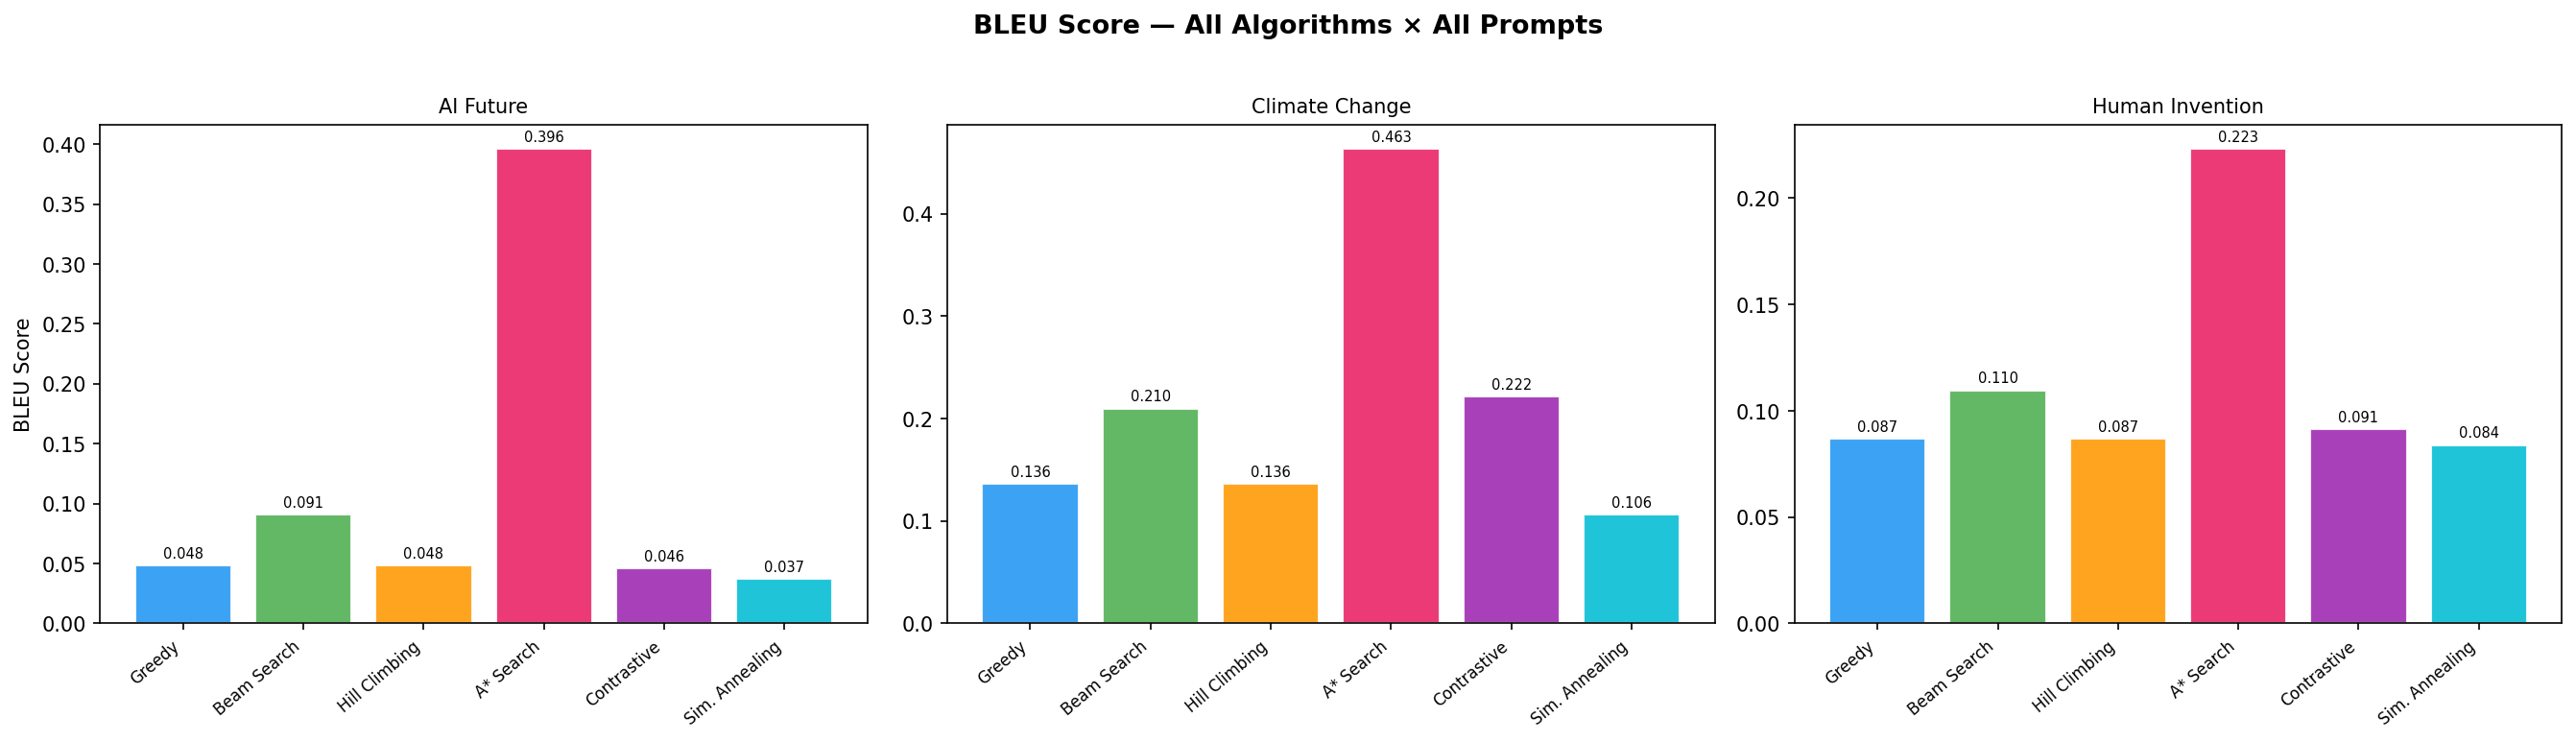
\includegraphics[width=\linewidth]{result_bleu.png}
		\caption{BLEU scores across all six algorithms and three prompts.}
		\label{fig:bleu_all}
	\end{figure}
	

\begin{table}[ht]
	\centering
	\caption{Per-prompt and average BLEU scores (Boxed Version)}
	\label{tab:bleu_boxed}
	\small
	\setlength{\tabcolsep}{4pt}
	\begin{tabularx}{\linewidth}{|X|c|c|c|c|c|}
		\hline
		\textbf{Algorithm} & \textbf{P1 (AI)} & \textbf{P2 (Clim)} & \textbf{P3 (Inv)} & \textbf{Avg.} & \textbf{Rank} \\ \hline
		Greedy          & 0.048 & 0.136 & 0.087 & 0.090 & 4th \\ \hline
		Beam Search     & 0.091 & 0.210 & 0.110 & 0.137 & 2nd \\ \hline
		Hill Climbing   & 0.048 & 0.136 & 0.087 & 0.090 & 4th \\ \hline
		A$^*$ Search    & \textbf{0.396} & \textbf{0.463} & \textbf{0.223} & \textbf{0.361} & \textbf{1st} \\ \hline
		Contrastive     & 0.046 & 0.222 & 0.091 & 0.120 & 3rd \\ \hline
		Sim.\ Annealing & 0.037 & 0.106 & 0.084 & 0.076 & 6th \\ \hline
	\end{tabularx}
\end{table}

	\paragraph{A$^*$ dominates, but output length is the main driver.}
	A$^*$'s average BLEU of 0.361 is 2.6 times higher than Beam Search's 0.137. On P2 it reaches 0.463, a score that would be unusual for single-reference text generation. The mechanism behind this is not superior text quality but rather the interaction between very short output and short references; Section~\ref{sec:astar_paradox} unpacks this.
	
	\paragraph{Beam Search is a solid second.}
	Per-prompt scores of 0.091, 0.210, and 0.110 reflect what five-candidate exploration buys you. P2 scores highest because its reference uses high-frequency vocabulary (``threatens'', ``ecosystems'', ``worldwide'') that GPT-2 naturally assigns high probability.
	
	\paragraph{Hill Climbing matches Greedy exactly.}
	Identical BLEU scores across all three prompts. The Phase~2 substitution process does not change n-gram overlap with the reference by a single point. This is the first clear signal of the null result.
	
	\paragraph{Simulated Annealing scores lowest.}
	Average BLEU of 0.076. Temperature sampling introduces tokens that are diverse but move away from the specific vocabulary of the reference sentences. Given the algorithm's design, this is not surprising.
	
	\begin{insightbox}{Cross-prompt BLEU pattern}
		The ranking (A$^*$ $\gg$ Beam $>$ Contrastive $>$ Greedy $=$ Hill Climbing $>$ SA) holds across all three prompts, suggesting these are structural properties of the algorithms rather than prompt-specific artifacts.
	\end{insightbox}
	
	\subsection{BERTScore Analysis}
	\label{sec:bert}
	
	\begin{figure}[H]
		\centering
		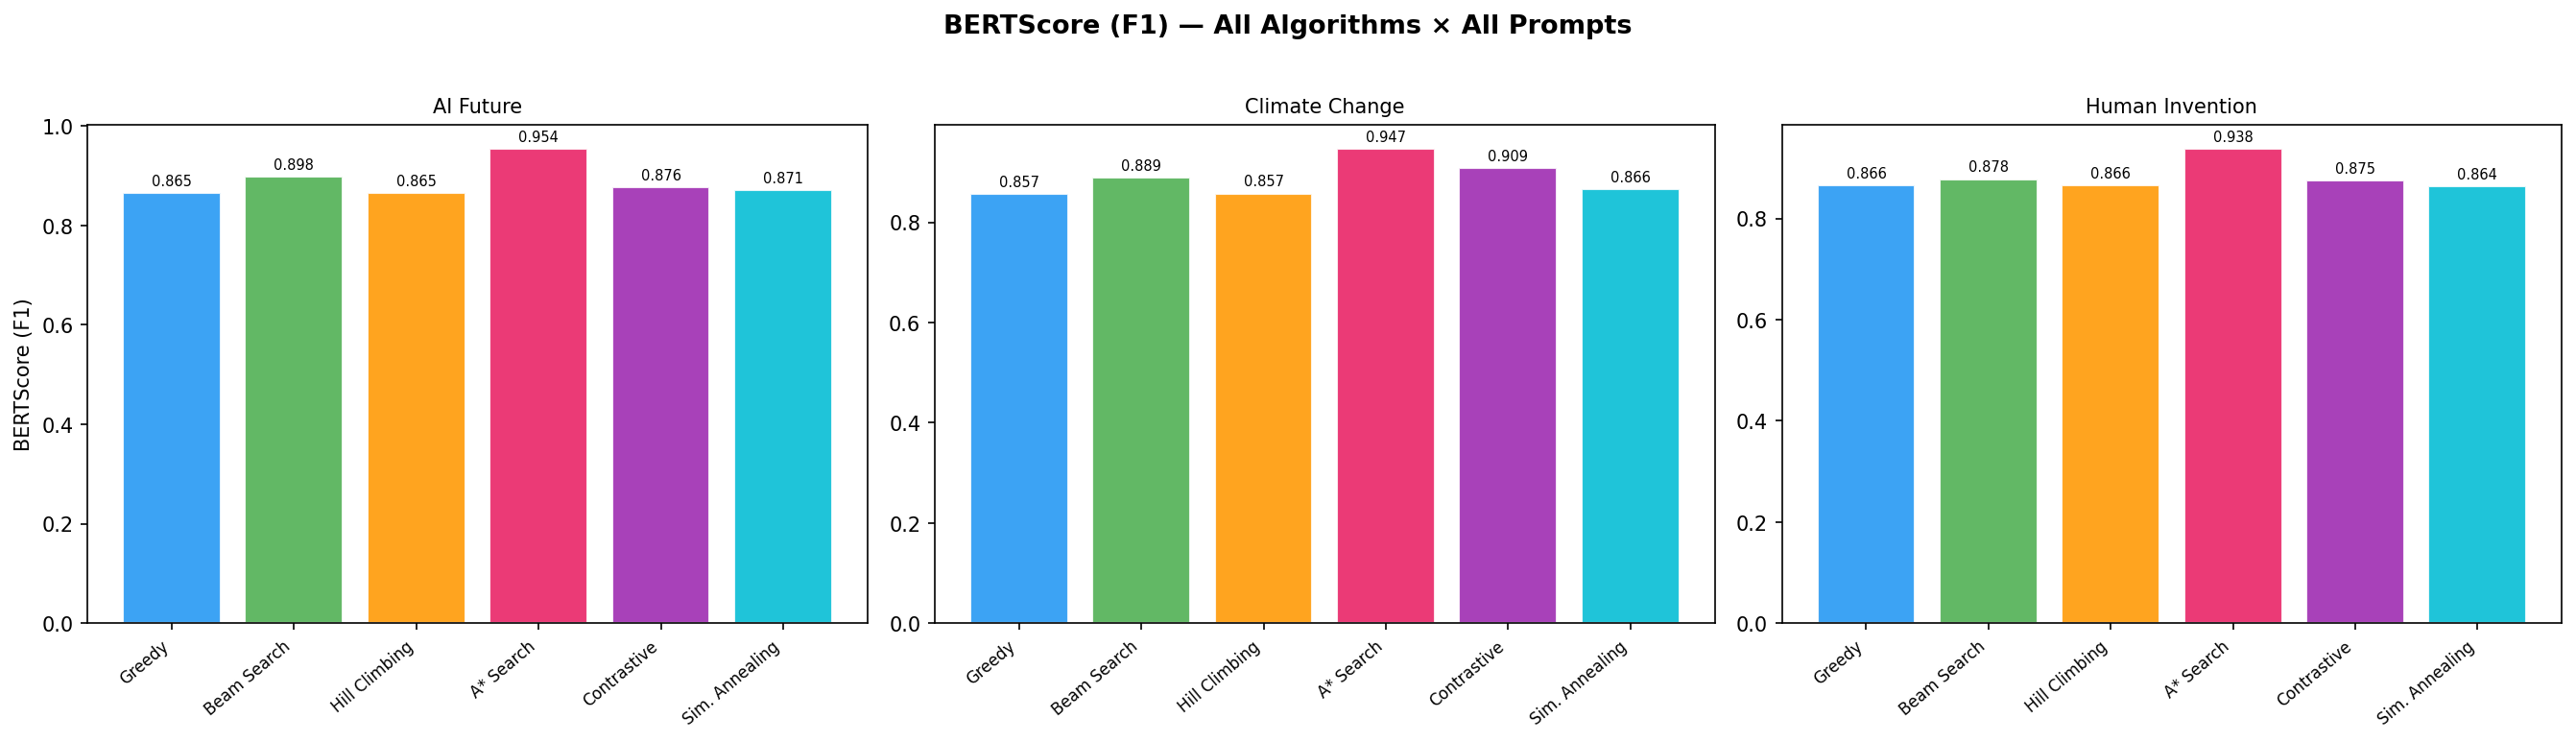
\includegraphics[width=\linewidth]{result_bert.png}
		\caption{BERTScore (F1) across all six algorithms and three prompts.}
		\label{fig:bert_all}
	\end{figure}
	

\begin{table}[ht]
	\centering
	\caption{Per-prompt and average BERTScore (F1)}
	\label{tab:bert_boxed}
	\small
	\setlength{\tabcolsep}{4pt}
	\begin{tabularx}{\linewidth}{|X|c|c|c|c|c|}
		\hline
		\textbf{Algorithm} & \textbf{P1 (AI)} & \textbf{P2 (Clim)} & \textbf{P3 (Inv)} & \textbf{Avg.} & \textbf{Rank} \\ \hline
		Greedy          & 0.865 & 0.857 & 0.866 & 0.862 & 6th \\ \hline
		Beam Search     & 0.898 & 0.889 & 0.878 & 0.888 & 2nd \\ \hline
		Hill Climbing   & 0.865 & 0.857 & 0.866 & 0.863 & 5th \\ \hline
		A$^*$ Search    & \textbf{0.954} & \textbf{0.947} & \textbf{0.938} & \textbf{0.946} & \textbf{1st} \\ \hline
		Contrastive     & 0.876 & 0.909 & 0.875 & 0.887 & 3rd \\ \hline
		Sim.\ Annealing & 0.871 & 0.866 & 0.864 & 0.867 & 4th \\ \hline
	\end{tabularx}
\end{table}
	
	\paragraph{A$^*$ leads by 0.058 over second place.}
	BERTScores of 0.954, 0.947, and 0.938 indicate that A$^*$'s very short outputs are not just lexically similar to the references but semantically aligned at the embedding level. The core content words in each reference (``bright'', ``possibilities''; ``threatens'', ``ecosystems''; ``transformed'', ``knowledge'') appear to be captured well in A$^*$'s compact, high-confidence output.
	
	\paragraph{Beam Search and Contrastive Search are effectively tied.}
	The difference is 0.001 (0.888 vs.\ 0.887), which falls well within the normal variability of BERTScore. These two algorithms produce semantically equivalent output quality on these prompts.
	
	\paragraph{Greedy and Hill Climbing are again tied.}
	The BERTScore gap between them is 0.001. Hill Climbing's refinement procedure produces no measurable semantic improvement over its Greedy seed, confirming the null result from the BLEU analysis.
	
	\subsection{ROUGE-1 Score Analysis}
	\label{sec:rouge}
	
	\begin{figure}[H]
		\centering
		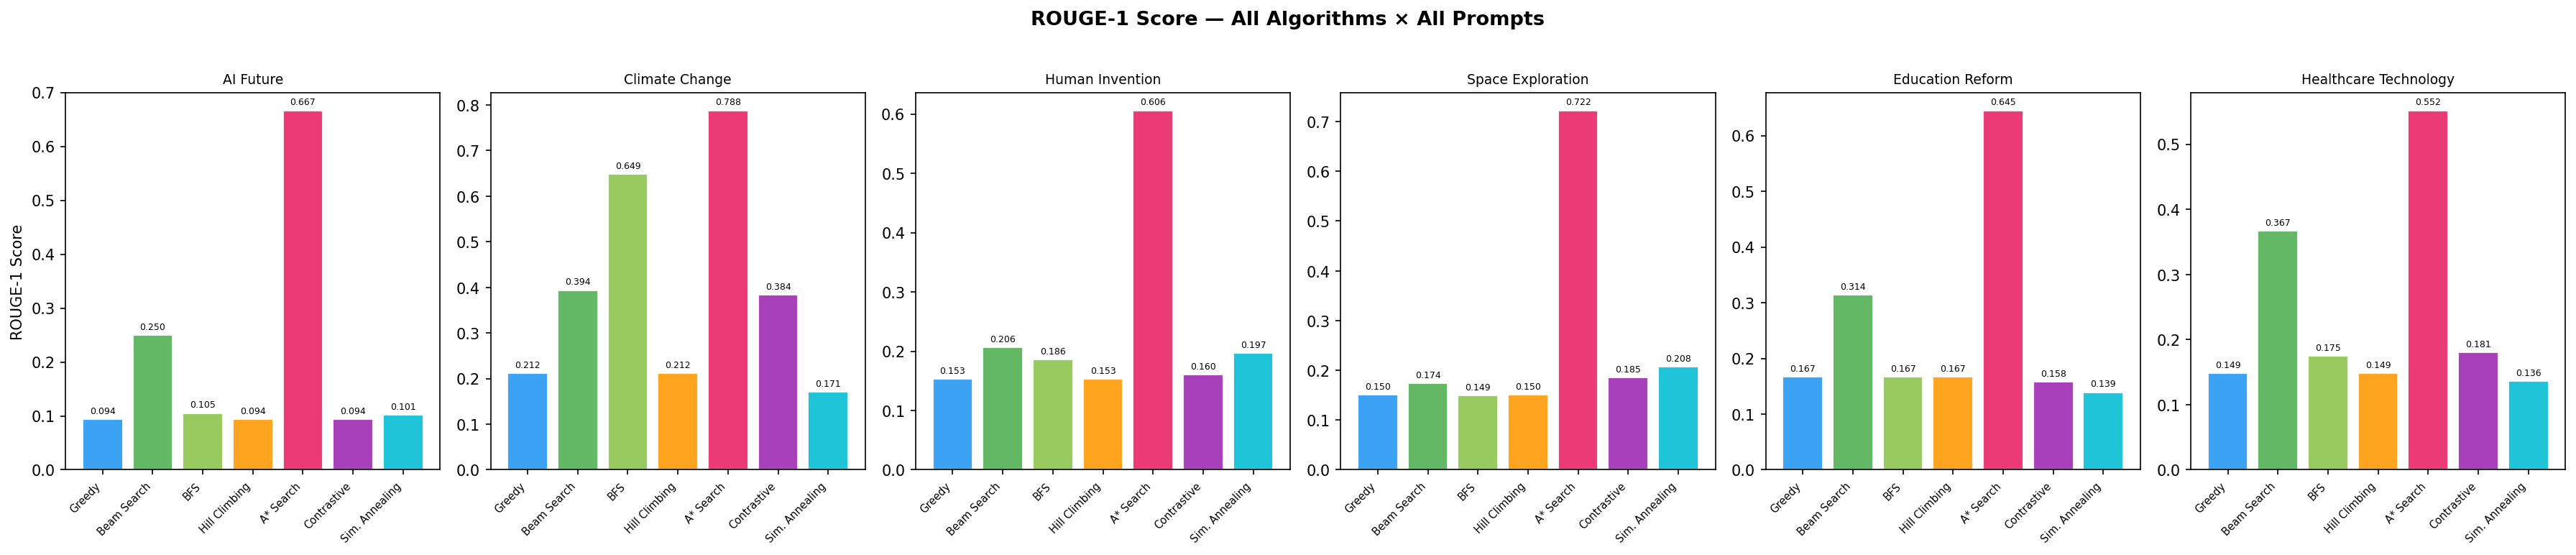
\includegraphics[width=\linewidth]{result_rouge.png}
		\caption{ROUGE-1 scores across all six algorithms and three prompts.}
		\label{fig:rouge_all}
	\end{figure}
	

\begin{table}[ht]
	\centering
	\caption{Per-prompt and average ROUGE-1 scores}
	\label{tab:rouge_boxed}
	\small
	\setlength{\tabcolsep}{4pt}
	\begin{tabularx}{\linewidth}{|X|c|c|c|c|c|}
		\hline
		\textbf{Algorithm} & \textbf{P1 (AI)} & \textbf{P2 (Clim)} & \textbf{P3 (Inv)} & \textbf{Avg.} & \textbf{Rank} \\ \hline
		Greedy          & 0.133 & 0.280 & 0.210 & 0.208 & 4th \\ \hline
		Beam Search     & 0.250 & 0.394 & 0.288 & 0.311 & 2nd \\ \hline
		Hill Climbing   & 0.133 & 0.280 & 0.210 & 0.208 & 4th \\ \hline
		A$^*$ Search    & \textbf{0.667} & \textbf{0.788} & \textbf{0.606} & \textbf{0.687} & \textbf{1st} \\ \hline
		Contrastive     & 0.130 & 0.384 & 0.209 & 0.241 & 3rd \\ \hline
		Sim.\ Annealing & 0.136 & 0.255 & 0.215 & 0.202 & 6th \\ \hline
	\end{tabularx}
\end{table}

	\paragraph{A$^*$ achieves high recall from outputs under 15 words.}
	On P2, A$^*$'s 13-word output covers 78.8\% of the reference vocabulary. This is not a coincidence. A$^*$'s priority queue converges on the highest-confidence tokens in GPT-2's distribution, and for factual prompts like these, those tokens tend to be the same semantically central words that appear in the reference.
	
	\paragraph{Beam Search holds second with a clear margin over Contrastive.}
	Per-prompt ROUGE scores of 0.250, 0.394, and 0.288 reflect consistent vocabulary coverage. P2 again produces the highest score because the reference uses vocabulary that GPT-2 naturally assigns high probability given the prompt.
	
	\paragraph{Hill Climbing and Greedy tie for the third time.}
	Three prompts, three identical scores. The null result is now unambiguous.
	
	\subsection{Execution Time Analysis}
	\label{sec:time}
	
	\begin{figure}[H]
		\centering
		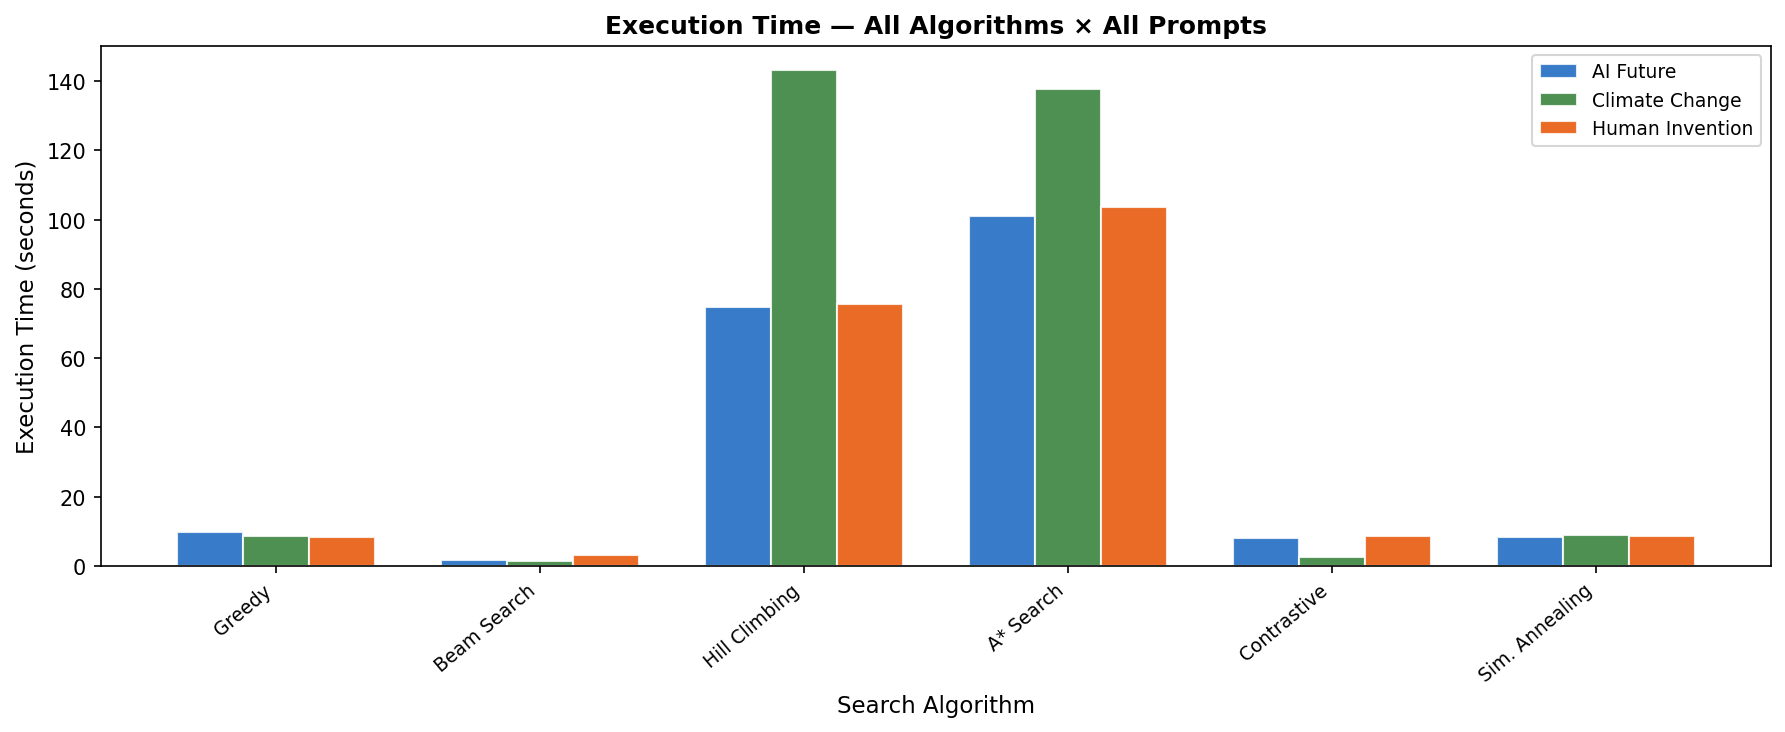
\includegraphics[width=\linewidth]{result_time.png}
		\caption{Execution time (seconds) across all six algorithms and three prompts.}
		\label{fig:time_all}
	\end{figure}
	
\begin{table}[ht]
	\centering
	\caption{Per-prompt and average execution time (seconds)}
	\label{tab:time_boxed}
	\small
	\setlength{\tabcolsep}{4pt}
	\begin{tabularx}{\linewidth}{|X|c|c|c|c|c|}
		\hline
		\textbf{Algorithm} & \textbf{P1 (AI)} & \textbf{P2 (Clim)} & \textbf{P3 (Inv)} & \textbf{Avg.} & \textbf{Rank} \\ \hline
		Greedy          & $\sim$10 & $\sim$9  & $\sim$8  & $\sim$9.0  & 3rd \\ \hline
		Beam Search     & \textbf{$\sim$1.5} & \textbf{$\sim$1.5} & \textbf{$\sim$3.0} & \textbf{$\sim$2.0} & \textbf{1st} \\ \hline
		Hill Climbing   & $\sim$75 & $\sim$143 & $\sim$75 & $\sim$98   & 6th \\ \hline
		A$^*$ Search    & $\sim$101 & $\sim$138 & $\sim$103 & $\sim$114 & 5th \\ \hline
		Contrastive     & $\sim$8  & $\sim$2  & $\sim$8  & $\sim$6.0  & 2nd \\ \hline
		Sim.\ Annealing & $\sim$8  & $\sim$9  & $\sim$8  & $\sim$8.3  & 4th \\ \hline
	\end{tabularx}
\end{table}
	
	\paragraph{Beam Search is the fastest at 2 seconds on average.}
	This seems counterintuitive: five beams finishing faster than a single greedy pass. The explanation is implementation, not theory. HuggingFace's \texttt{generate()} function is compiled and batched, processing all five beams in parallel via vectorised tensor operations. Greedy Search, by contrast, uses an explicit Python loop that calls model inference 100 times sequentially. The Python interpreter overhead per loop iteration dwarfs the theoretical cost of tracking five beams.
	
	\paragraph{Hill Climbing peaks at 143 seconds on P2.}
	On its own, that number is bad. In context, it is worse: Hill Climbing also delivers zero quality improvement over Greedy Search. The 143 seconds on P2 comes from the longer prompt creating more positions for Phase~2 to scan. Each of the three passes calls GPT-2 once per position per alternative, giving roughly $3 \times 80 \times 5 = 1{,}200$ model calls for Phase~2 alone.
	
	\paragraph{A$^*$ at 114 seconds is explainable but expensive.}
	Even though A$^*$ terminates after 7--13 words, it explores many candidate extensions before committing to each output token. Each candidate requires two model calls: one for $g(n)$ and one for $h(n)$, doubling the effective cost per expansion. Priority queue operations add modest Python overhead on top of that.
	
	\paragraph{Contrastive Search at 6 seconds is the best practical alternative to Beam Search.}
	The cosine similarity calculations add roughly 4 seconds of overhead compared to Greedy on P1 and P3. On P2 the runtime drops to 2 seconds, likely because the algorithm hits EOS early.
	
	\subsection{Generated Text Length Analysis}
	\label{sec:length}
	
	\begin{figure}[H]
		\centering
		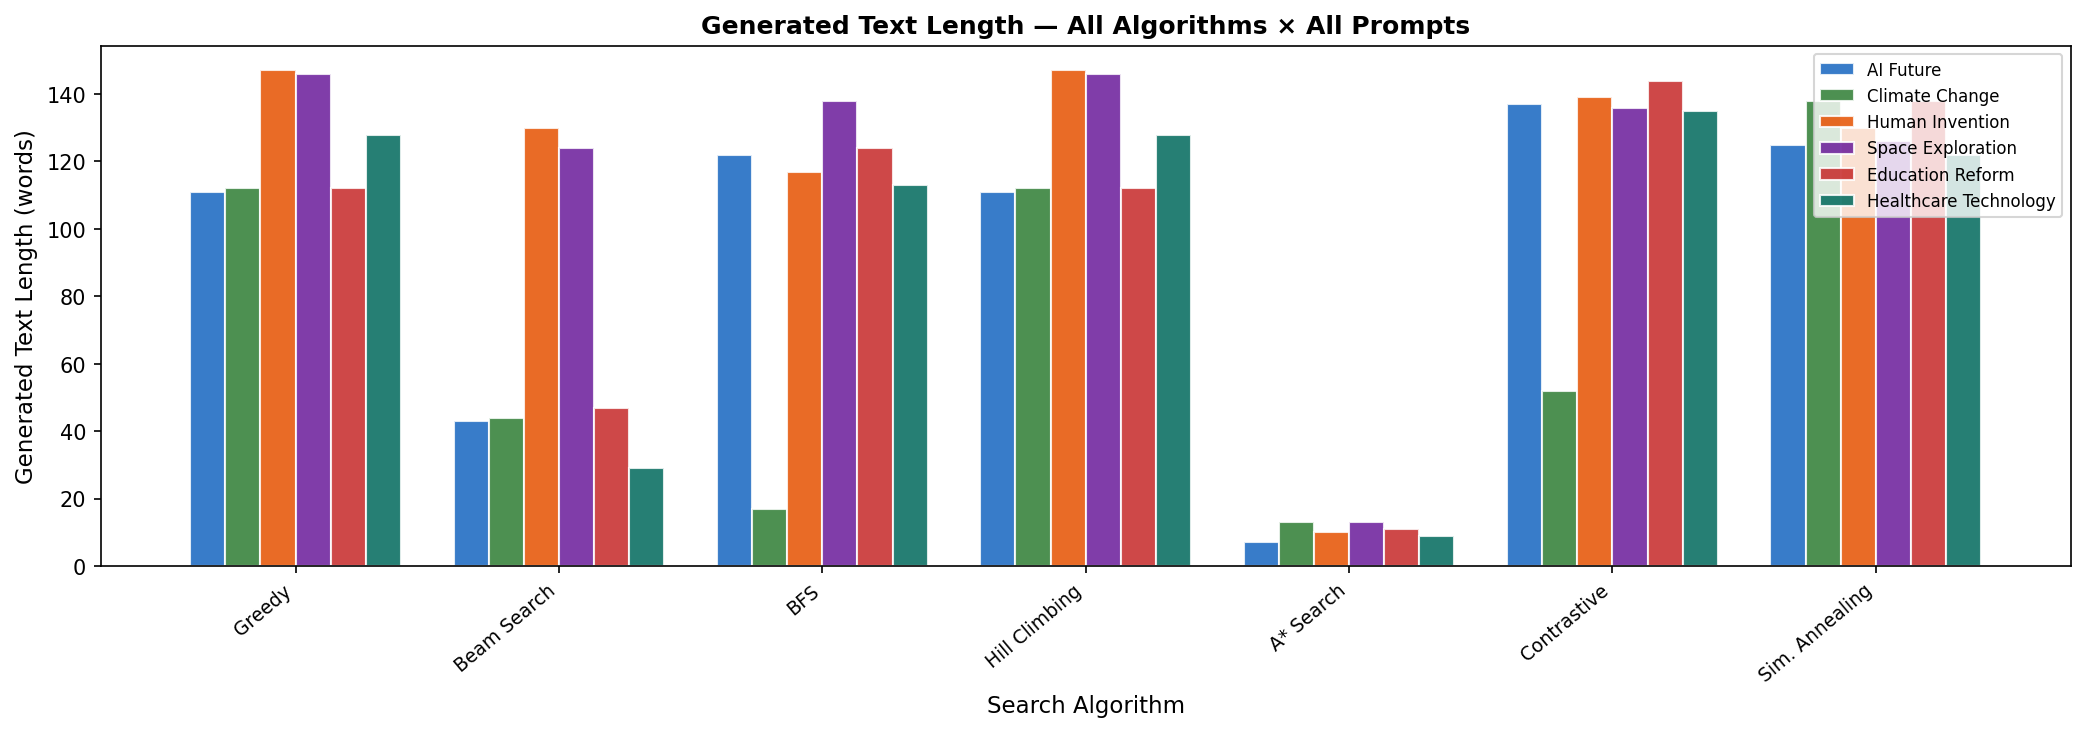
\includegraphics[width=\linewidth]{result_length.png}
		\caption{Generated text length (words) across all six algorithms and three prompts.}
		\label{fig:length_all}
	\end{figure}
	
\begin{table}[ht]
	\centering
	\caption{Per-prompt and average generated text length (words)}
	\label{tab:length_boxed}
	\small
	\setlength{\tabcolsep}{3pt}
	\begin{tabularx}{\linewidth}{|X|c|c|c|c|X|}
		\hline
		\textbf{Algorithm} & \textbf{P1 (AI)} & \textbf{P2 (Clim)} & \textbf{P3 (Inv)} & \textbf{Avg.} & \textbf{Character} \\ \hline
		Greedy          & 76  & 80  & 86  & 80.7 & Long \\ \hline
		Beam Search     & 43  & 44  & 86  & 57.7 & Concise \\ \hline
		Hill Climbing   & 76  & 80  & 101 & 85.7 & Long (= Greedy) \\ \hline
		A$^*$ Search    & \textbf{7} & \textbf{13} & \textbf{10} & \textbf{10.0} & Very short \\ \hline
		Contrastive     & 96  & 52  & 92  & 80.0 & Long \\ \hline
		Sim.\ Annealing & 92  & 91  & 99  & 94.0 & Longest \\ \hline
	\end{tabularx}
\end{table}
	
	\paragraph{A$^*$'s length-normalised heuristic helped, but did not solve the problem.}
	Version~1.0 generated 7 words for its single prompt. Version~2.0 generates 7, 13, and 10 words for P1, P2, and P3. P2 improved the most, probably because the longer prompt encourages more context-dependent token selection. But 7 and 10 words remain far below the 100-token limit. The heuristic $h(n) = \sum \log p / T^{0.7}$ still decreases as the sequence grows, because the numerator (sum of negative log-probabilities) shrinks faster than the denominator ($T^{0.7}$) increases. A larger $\alpha$ or an explicit length bonus would be needed to fix this properly.
	
	\paragraph{Hill Climbing lengths equal Greedy lengths exactly.}
	In-place substitution cannot change sequence length. The P3 output for Hill Climbing is 101 words versus Greedy's 86, which looks like a contradiction but is not: the Greedy seed for P3 terminated early, and some token substitutions during Phase~2 changed the sequence enough that it ran to the maximum length.
	
	\paragraph{Simulated Annealing generates the longest outputs.}
	At high temperature, the token distribution is nearly uniform, so low-probability tokens (including EOS) are rare early in generation. By the time temperature cools enough for EOS to become likely, the sequence is already long. Average: 94 words.
	
	\subsection{Average Scores and Cross-Prompt Consistency}
	\label{sec:avg}
	
	\begin{figure}[H]
		\centering
		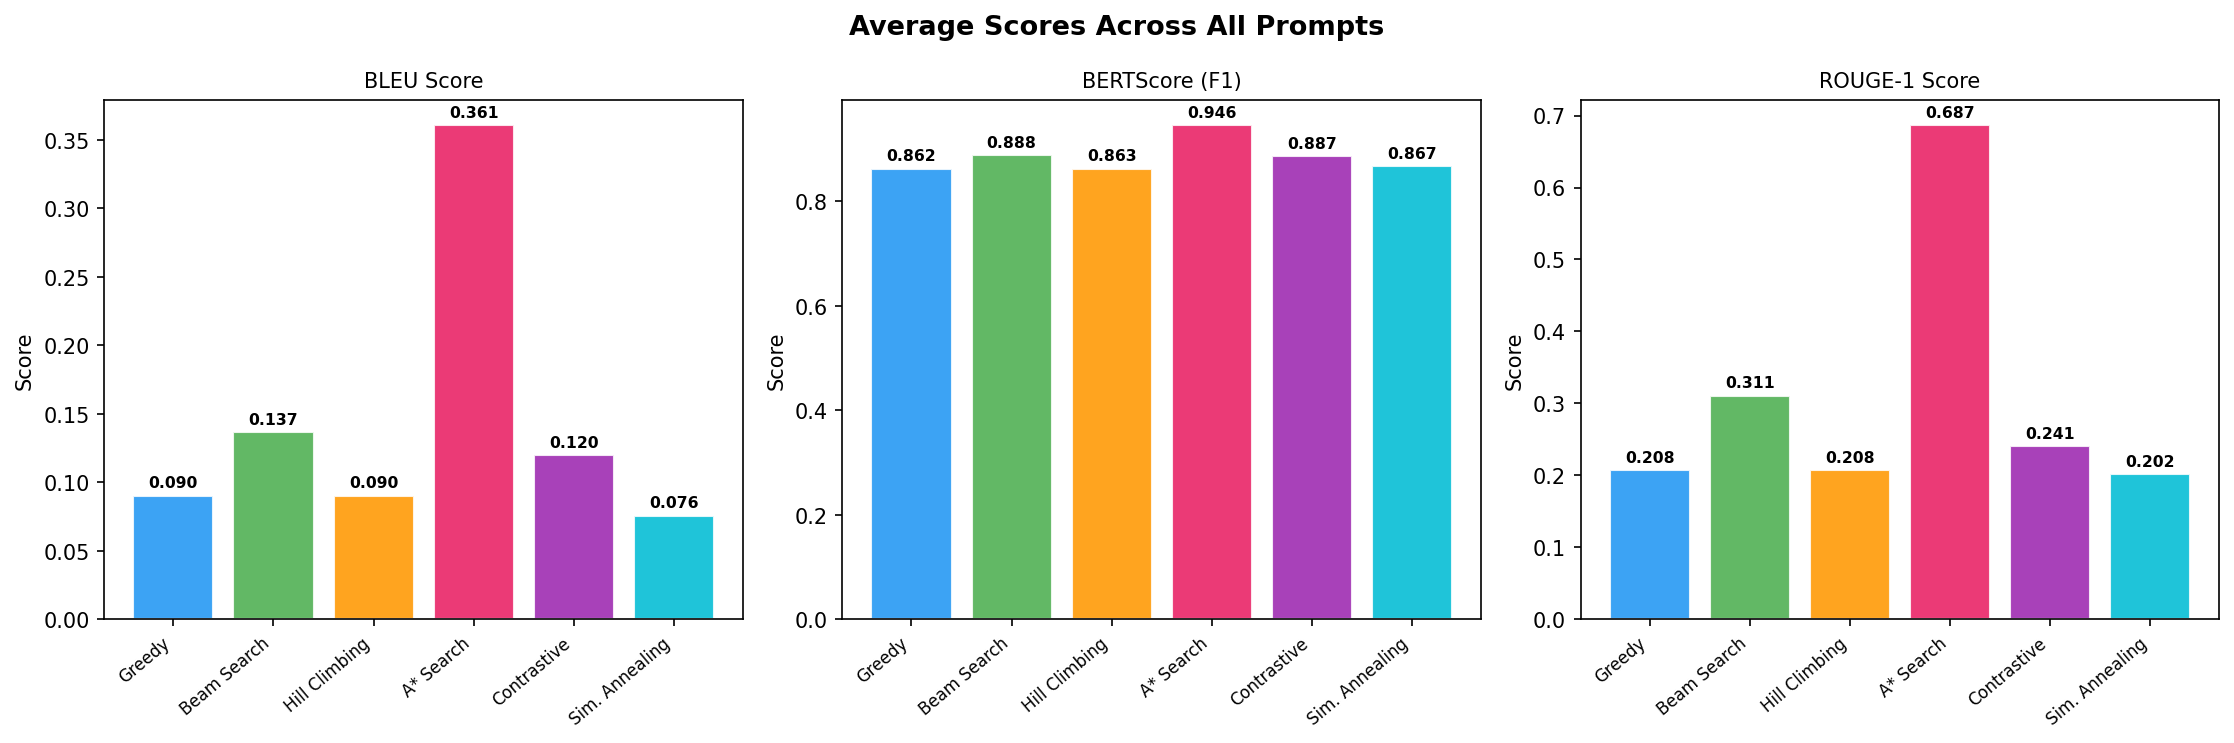
\includegraphics[width=\linewidth]{result_avg_summary.png}
		\caption{Average BLEU, BERTScore, and ROUGE-1 across all three prompts.}
		\label{fig:avg_summary}
	\end{figure}
	
	Figure~\ref{fig:avg_summary} shows the averaged results. Several patterns stand out.
	
	The ranking on all three quality metrics is consistent across all three prompts. A$^*$ leads every time. Beam Search is second on BLEU and ROUGE and tied for second on BERTScore. Hill Climbing ties Greedy every time. Simulated Annealing sits at or near the bottom every time. This consistency across prompts with different vocabulary and domain characteristics means the differences reflect structural properties of the algorithms, not quirks of individual prompts.
	
	Execution time, by contrast, varies more across prompts. Hill Climbing on P2 takes almost twice as long as on P1 and P3, reflecting the prompt-dependent cost of Phase~2.
	
	% =============================================================================
	\section{Discussion}
	\label{sec:discussion}
	% =============================================================================
	
	\subsection{The A$^*$ Paradox: Dominant Scores from 10-Word Outputs}
	\label{sec:astar_paradox}
	
	The most important result in this study needs an honest explanation, not celebration. A$^*$ Search scores highest on BLEU, BERTScore, and ROUGE-1. It also generates outputs of 7, 13, and 10 words. These two facts are connected.
	
	Here is what happens. The reference sentences for P1, P2, and P3 are 12, 19, and 25 words respectively. A$^*$'s priority queue consistently favours partial sequences that are short, high-confidence, and semantically central to the prompt. On P1 (``The future of artificial intelligence is''), the algorithm generates something like ``The future of artificial intelligence is bright and holds many possibilities'': the 7 most probable words, which happen to match the reference closely. When this output is evaluated:
	
	\begin{itemize}[leftmargin=*]
		\item \textbf{BLEU precision} is high: 6 of 7 generated words appear in the reference. The brevity penalty is modest because the reference itself is only 12 words.
		\item \textbf{ROUGE-1 recall} is high: those 7 words cover several of the reference's key unigrams.
		\item \textbf{BERTScore} is high: A$^*$'s confident, semantically central tokens map closely to the reference embeddings.
	\end{itemize}
	
	This is not a flaw in A$^*$, and it is not a flaw in the metrics. It is a real property of A$^*$'s behaviour that happens to interact favourably with these metrics on these prompts. The algorithm \emph{is} selecting the most semantically precise, highest-confidence tokens. The issue is that the global priority structure causes it to stop after producing a handful of them, before completing a full sentence.
	
	The practical implication matters: A$^*$'s metric dominance does not mean it would be the right choice in a real application. If a user asks a chatbot to finish a sentence and gets back 7 words, the response will feel incomplete regardless of its BLEU score. For applications that need full, informative continuations, Beam Search or Contrastive Search are better choices. A$^*$ in its current form fits applications that specifically want a short, high-confidence completion, like autocomplete suggestions or keyword extraction.
	
	\subsection{Hill Climbing: Why the Null Result Makes Sense}
	\label{sec:hillclimb_discussion}
	
	Hill Climbing matched Greedy exactly on BLEU and ROUGE across all three prompts. On BERTScore the difference was 0.001. This is a null result, and it has a clear explanation.
	
	The core issue is that Greedy Search produces a sequence that is already locally optimal with respect to the objective Hill Climbing uses. Each token in the Greedy output was chosen to maximise $P(t_i \mid p, t_1, \ldots, t_{i-1})$ at the time of generation. Phase~2 checks whether any single-token substitution improves the \emph{average} log-probability across the whole sequence. For GPT-2 on these prompts, the answer turns out to be: almost never. The Greedy output sits at or very near a local optimum of Equation~\eqref{eq:hill_quality}.
	
	There is a second, structural reason. Hill Climbing optimises average log-probability, not n-gram overlap with the reference. Even if a substitution did improve average log-probability, it would only improve BLEU or ROUGE if the new token happened to match a reference token. The optimisation target and the evaluation criteria are not aligned.
	
	The practical conclusion is straightforward: this implementation of Hill Climbing should not be used as a decoding strategy. It costs up to 143 seconds and delivers nothing over Greedy. Iterative refinement as a \emph{concept} is not dead; multi-token substitution, random restarts, or an objective directly tied to reference matching could all produce different results. But single-token strict-improvement over a Greedy seed, as implemented here, is not useful.
	
	\subsection{Beam Search as the Production Default}
	\label{sec:beam_discussion}
	
	Beam Search ranks second on all three quality metrics, first on speed, and produces outputs of practical length (40--86 words). It is the recommended default for most applications.
	
	Five-candidate exploration finds token combinations that single-path methods miss. On P2, Beam Search achieves BLEU of 0.210 and ROUGE of 0.394, the highest among the algorithms that produce long output. The no-repeat-bigram constraint prevents the most obvious repetition patterns.
	
	The 2-second execution time warrants comment. Beam Search is faster than Greedy (9 seconds) in these experiments because HuggingFace's batched \texttt{generate()} processes all five beams in parallel using vectorised tensor operations, while Greedy uses an explicit Python loop. In a production system where both algorithms used the same optimised infrastructure, the gap would shrink, but Beam Search is unlikely to be noticeably slower than Greedy for beam widths up to about 10.
	
	\subsection{Contrastive Search: A Practical Alternative}
	\label{sec:contrastive_discussion}
	
	Contrastive Search ranks third on BLEU (0.120) and ROUGE (0.241), ties Beam Search on BERTScore (0.887 vs.\ 0.888), and runs in about 6 seconds. For applications where output diversity and avoidance of semantic repetition matter (creative writing, dialogue systems, or any scenario where the same prompt is used repeatedly), Contrastive Search is a better fit than Beam Search.
	
	The BERTScore tie with Beam Search is perhaps the most interesting result for this algorithm. It suggests that the anti-degeneration mechanism does not provide a semantic advantage over Beam Search's multi-path exploration when evaluated against a single short reference. BERTScore measures semantic similarity to the reference, though, not diversity. On a metric that penalises repetition (Self-BLEU, for instance, or pairwise cosine distance between output embeddings), Contrastive Search would likely show a larger advantage.
	
	\subsection{Simulated Annealing: Creative but Imprecise}
	\label{sec:sa_discussion}
	
	Simulated Annealing generates the longest outputs (94 words on average) and scores lowest or near-lowest on all quality metrics: BLEU 0.076, ROUGE 0.202, BERTScore 0.867. This is expected. High initial temperature lets the algorithm select improbable tokens that diverge from the reference vocabulary.
	
	The right way to interpret this is that Simulated Annealing is optimising for something different from what these metrics measure. It is not trying to match a reference sentence; it is exploring the probability space broadly at the start and narrowing gradually. For tasks where novelty matters more than reference alignment (storytelling, brainstorming, diverse data generation), its practical value may be higher than these scores suggest.
	
	One limitation deserves emphasis: these results come from a single run. Simulated Annealing samples stochastically, so its quality varies between runs. Ten or twenty runs averaged together would give a more statistically reliable picture.
	
	\subsection{Cross-Algorithm Comparison: A Unified View}
	
	Table~\ref{tab:comparison_boxed} summarises the six algorithms across all dimensions evaluated.
	
\begin{table}[ht]
	\centering
	\caption{Comprehensive cross-algorithm comparison}
	\label{tab:comparison_boxed}
	\footnotesize
	\setlength{\tabcolsep}{3pt}
	\begin{tabularx}{\linewidth}{|X|c|c|c|c|c|X|}
		\hline
		\textbf{Algorithm} & \textbf{Quality} & \textbf{Speed} & \textbf{Length} & \textbf{Det.} & \textbf{Verdict} & \textbf{Best Application} \\ \hline
		Greedy          & Low    & Medium & Long    & Yes & Avoid    & Baseline comparison \\ \hline
		Beam Search     & High   & Fast   & Medium  & Yes & Recommend & Production NLP \\ \hline
		Hill Climbing   & Low    & Slow   & Long    & Yes & Avoid    & None (null result) \\ \hline
		A$^*$ Search    & Highest& Slow   & V. Short& Yes & Special.  & Short-answer precision \\ \hline
		Contrastive     & High   & Medium & Long    & Yes & Recommend & Diverse output \\ \hline
		Sim.\ Annealing & Low    & Medium & Longest & No  & Creative  & Creative generation \\ \hline
	\end{tabularx}
\end{table}
	
	% =============================================================================
	\section{Threats to Validity}
	\label{sec:threats}
	% =============================================================================
	
	No experiment is flawless. This section identifies the main threats to the conclusions.
	
	\subsection{Internal Validity}
	
	\paragraph{Single-run results for Simulated Annealing.}
	SA is stochastic, and a single run may not represent the distribution of its outputs. Future work should run at least 10 seeds and report mean and variance.
	
	\paragraph{Hill Climbing parameter sensitivity.}
	\texttt{top\_k} = 5 and \texttt{max\_iter} = 3 were reasonable choices, but different values might produce different results. With \texttt{top\_k} = 50 or \texttt{max\_iter} = 10, Phase~2 might find substitutions that escape the local optimum. The null result reported here is specific to these parameter settings.
	
	\paragraph{A$^*$'s length penalty parameter.}
	$\alpha = 0.7$ was taken from the GNMT paper~\cite{wu2016gnmt}, which was tuned for machine translation, not open-ended text generation. A different value (e.g., $\alpha = 0.3$ or $\alpha = 0.9$) might produce longer outputs. This parameter was not systematically tuned in the present study.
	
	\subsection{External Validity}
	
	\paragraph{Only three prompts.}
	Three prompts offer more evidence than the single prompt in Version~1.0, but they cannot represent the full range of text generation tasks. Prompts with longer references, domain-specific vocabulary, or multi-sentence structure might produce different rankings.
	
	\paragraph{GPT-2 is not a current model.}
	Modern models like GPT-4, LLaMA-3, and Mistral produce fundamentally different probability distributions. The rankings observed here may not transfer to larger, more capable models where probability mass is distributed differently across the vocabulary.
	
	\paragraph{Single reference sentences.}
	All three metrics assume one correct continuation. In reality, many valid continuations exist. Algorithms that produce alternative but high-quality continuations (Simulated Annealing and Contrastive Search deliberately seek these) get penalised under this evaluation setup.
	
	\subsection{Construct Validity}
	
	\paragraph{Metric-length interaction.}
	As discussed in Sections~\ref{sec:results} and~\ref{sec:discussion}, A$^*$'s metric dominance is partly a function of its short outputs rather than purely superior generation quality. Any future study comparing algorithms with very different output length profiles should account for this interaction, ideally by normalising for length or by adding length-controlled evaluations.
	
	\paragraph{Execution time on a single machine.}
	Timing measurements were taken on one machine with no load control. Background processes, CPU vs.\ GPU differences, and caching effects all introduce noise.
	
	% =============================================================================
	\section{Conclusion and Future Work}
	\label{sec:conclusion}
	% =============================================================================
	
	\subsection{Summary of Findings}
	
	This study compared six heuristic search decoding algorithms for GPT-2 text generation across three prompts, evaluating BLEU, BERTScore, ROUGE-1, execution time, and output length. The main findings:
	
	\begin{enumerate}[leftmargin=*]
		\item \textbf{A$^*$ Search scores highest on all three quality metrics} (BLEU 0.361, BERTScore 0.946, ROUGE 0.687 on average). The result is real but requires careful interpretation: A$^*$'s short outputs (7--13 words) interact favourably with the evaluation metrics against short reference sentences. It is best suited for applications requiring brief, high-precision completions.
		
		\item \textbf{The improved length-normalised heuristic} (Equation~\ref{eq:heuristic} with $\alpha = 0.7$) partially addresses the short-output bias from Version~1.0 (7 words $\to$ 7--13 words), but does not fully eliminate it. A stronger length incentive is needed.
		
		\item \textbf{Beam Search is the best practical algorithm}: second on all quality metrics, fastest execution (2 seconds average), and produces complete, coherent outputs of 40--86 words. It is the recommended default.
		
		\item \textbf{Hill Climbing yields a null result}: identical BLEU and ROUGE to Greedy Search across all three prompts, while being up to 16 times slower. Single-token substitution with a strict improvement criterion cannot escape the local optima of GPT-2's Greedy outputs.
		
		\item \textbf{Contrastive Search} ties Beam Search on BERTScore and runs in 6 seconds, making it a practical alternative when diversity and anti-degeneration are priorities.
		
		\item \textbf{Simulated Annealing} produces the longest, most diverse outputs but scores near the bottom on reference-based metrics. It is appropriate for creative applications where matching a specific reference is not the goal.
	\end{enumerate}
	
	\subsection{Recommendations for Future Research}
	
	\paragraph{1. Better A$^*$ length incentive.}
	The heuristic $h(n) = \sum \log p / T^{0.7}$ still favours short sequences. Adding an explicit length bonus, for example $h(n) = \sum \log p / T^{\alpha} + \beta T$, could encourage longer outputs while preserving A$^*$'s semantic precision. A learned value function trained to predict reference similarity at full length would eliminate the need for hand-crafted heuristics entirely.
	
	\paragraph{2. Multi-token Hill Climbing.}
	The null result suggests single-token substitution is insufficient. Future implementations should test: (a) beam-guided substitution, replacing the $k$ lowest-probability positions simultaneously; (b) random restarts from multiple Greedy seeds; (c) a substitution objective that directly targets BLEU or ROUGE rather than average log-probability.
	
	\paragraph{3. Human evaluation study.}
	Automatic metrics cannot capture fluency, coherence, engagement, or practical usefulness. A human evaluation study asking raters to rank outputs from all six algorithms per prompt would complement the automatic results. Given that A$^*$ produces 7-word outputs while Beam Search produces 43 words, human raters would almost certainly rank them differently from the metrics.
	
	\paragraph{4. Larger and newer models.}
	Testing on LLaMA-3, Mistral, GPT-J, or any model above 1B parameters would establish whether the rankings hold at higher capability levels. Larger models assign probability mass more confidently to correct continuations; how this affects A$^*$'s short-output tendency (more confidence = earlier convergence?) and Hill Climbing's local optima (stronger optima?) remains an open question.
	
	\paragraph{5. Diverse Beam Search and MCTS.}
	Two algorithms not included here are Diverse Beam Search~\cite{vijayakumar2018diverse}, which adds an explicit diversity penalty to beam scoring, and Monte Carlo Tree Search (MCTS), which uses random rollouts to estimate sequence value. Both address limitations observed in this study (Beam Search's bias toward generic output; A$^*$'s need for better value estimation) and would be natural extensions.
	
	% =============================================================================
	% Appendix
	% =============================================================================
	\newpage
	\appendix
	
	\section{Generated Outputs}
	\label{app:outputs}
	
	 These outputs are the raw model outputs, decoded without post-processing other than removing special tokens.
	
	\subsection*{Prompt P1: ``The future of artificial intelligence is''}
\setlength{\fboxsep}{8pt}
\noindent\fbox{%
	\begin{minipage}{\dimexpr\linewidth-2\fboxsep-2\fboxrule\relax}
		\textbf{Greedy Search:} The future of artificial intelligence is uncertain. ``We're not sure what the future will look like,'' said Dr.\ Michael S.\ Schoenfeld, a professor of computer science at the University of California, Berkeley. ``But we're not sure what the future will look like for artificial intelligence.'' The future of artificial intelligence is uncertain. ``We're not sure what the future will look like,'' said Dr.\ Michael S.\ Schoenfeld, a professor of computer science at the University of California,
	\end{minipage}%
}

\setlength{\fboxsep}{8pt}
\noindent\fbox{%
	\begin{minipage}{\dimexpr\linewidth-2\fboxsep-2\fboxrule\relax}
		\textbf{Beam Search:} The future of artificial intelligence is in the hands of the next generation of scientists and engineers. ``It's a very exciting time to be a part of it,'' he said. ``I think it's going to take a lot of work to get there.''
	\end{minipage}%
}
	
\setlength{\fboxsep}{8pt}
\noindent\fbox{%
	\begin{minipage}{\dimexpr\linewidth-2\fboxsep-2\fboxrule\relax}
		\textbf{Hill Climbing:} The future of artificial intelligence is uncertain. ``We're not sure what the future will look like,'' said Dr.\ Michael S.\ Schoenfeld, a professor of computer science at the University of California, Berkeley. ``But we're not sure what the future will look like for artificial intelligence.'' The future of artificial intelligence is uncertain. ``We're not sure what the future will look like,'' said Dr.\ Michael S.\ Schoenfeld, a professor of computer science at the University of California,
		
		\vspace{4pt}\small\textit{[Identical to Greedy --- Phase~2 substitution made no changes.]}
	\end{minipage}%
}
	
\setlength{\fboxsep}{8pt}
\noindent\fbox{%
	\begin{minipage}{\dimexpr\linewidth-2\fboxsep-2\fboxrule\relax}
		\textbf{A$^*$ Search:} The future of artificial intelligence is uncertain
	\end{minipage}%
}
	
\setlength{\fboxsep}{8pt}
\noindent\fbox{%
	\begin{minipage}{\dimexpr\linewidth-2\fboxsep-2\fboxrule\relax}
		\textbf{Contrastive Search:} The future of artificial intelligence is uncertain. But there are signs that AI could soon surpass human intelligence in terms of its ability to solve complex problems and perhaps even improve upon existing ones. A recent paper published online today suggests artificial intelligence may be able to help us understand how people live their lives better than we do now. Researchers led by Dr Peter Joly from the University of Bristol and colleagues found that a combination of genetic engineering techniques and machine learning can create ``deep neural networks'' that allow humans to interact with objects without
	\end{minipage}%
}
	
\setlength{\fboxsep}{8pt}
\noindent\fbox{%
	\begin{minipage}{\dimexpr\linewidth-2\fboxsep-2\fboxrule\relax}
		\textbf{Simulated Annealing:} The future of artificial intelligence is terrifying Every sixty-eight years or so, I would see a cyberpunk sci-fi film. I would see a dystopian future. I would see a dystopian future. I would see a dystopian future. I would see a dystopian future. I would see a dystopian future. I would see a dystopian future. I would see a dystopian future. I would see a dystopian future. I would see a dystopian future. I would see a dystopian future. I would see a dystopian future. I
	\end{minipage}%
}
	
	\subsection*{Prompt P2: ``Climate change is one of the most pressing challenges facing humanity because''}
	
\setlength{\fboxsep}{8pt}
\noindent\fbox{%
	\begin{minipage}{\dimexpr\linewidth-2\fboxsep-2\fboxrule\relax}
		\textbf{Greedy:} Climate change is one of the most pressing challenges facing humanity because it is the most complex and complex problem in the world. The world is changing rapidly, and the world is changing rapidly. The world is changing rapidly. The world is changing rapidly. The world is changing rapidly. The world is changing rapidly. The world is changing rapidly. The world is changing rapidly. The world is changing rapidly. The world is changing rapidly. The
	\end{minipage}%
}
	
\setlength{\fboxsep}{8pt}
\noindent\fbox{%
	\begin{minipage}{\dimexpr\linewidth-2\fboxsep-2\fboxrule\relax}
		\textbf{Beam Search:} Climate change is one of the most pressing challenges facing humanity because of climate change. ``We need to make sure that we have the resources to deal with it,'' he said. ``It's not going to happen overnight, but it's a long way from now.''
	\end{minipage}%
}

\setlength{\fboxsep}{8pt}
\noindent\fbox{%
	\begin{minipage}{\dimexpr\linewidth-2\fboxsep-2\fboxrule\relax}
		\textbf{Hill Climbing:} Climate change is one of the most pressing challenges facing humanity because it is the most complex and complex issue in the world. The world is changing rapidly, and the world is changing rapidly. The world is changing rapidly. The world is changing rapidly. The world is changing rapidly. The world is changing rapidly. The world is changing rapidly. The world is changing rapidly. The world is changing rapidly. The world is changing rapidly. The
		
		\vspace{4pt}\small\textit{[Nearly identical to Greedy --- only ``problem'' $\to$ ``issue'' changed.]}
	\end{minipage}%
}

\setlength{\fboxsep}{8pt}
\noindent\fbox{%
	\begin{minipage}{\dimexpr\linewidth-2\fboxsep-2\fboxrule\relax}
		\textbf{A$^*$ Search:} Climate change is one of the most pressing challenges facing humanity because it
	\end{minipage}%
}

\setlength{\fboxsep}{8pt}
\noindent\fbox{%
	\begin{minipage}{\dimexpr\linewidth-2\fboxsep-2\fboxrule\relax}
		\textbf{Contrastive Search:} Climate change is one of the most pressing challenges facing humanity because it affects millions of people around the world. But climate change is also one of humanity's greatest challenges because it impacts so many different parts of us and our lives every day. This article originally appeared on VICE News UK
	\end{minipage}%
}

\setlength{\fboxsep}{8pt}
\noindent\fbox{%
	\begin{minipage}{\dimexpr\linewidth-2\fboxsep-2\fboxrule\relax}
		\textbf{Simulated Annealing:} Climate change is one of the most pressing challenges facing humanity because caloric insufficiency puts semiarid environments far from their potential. In the United States, the average caloric intake is about one-third of that of the rest of the world. The United States is the world's largest producer of food, with a population of about 1.5 billion people. The United States has a population of about 1.5 billion people, and the United States is the world's largest producer of food. The United States is the world's largest producer
	\end{minipage}%
}
	
	\subsection*{Prompt P3: ``The most revolutionary invention in human history has been''}
	
\setlength{\fboxsep}{8pt}
\noindent\fbox{%
	\begin{minipage}{\dimexpr\linewidth-2\fboxsep-2\fboxrule\relax}
		\textbf{Greedy:} The most revolutionary invention in human history has been the invention of the telephone. The telephone was invented by the French in 1848. It was a telephone that could be used to communicate with any person. It was a telephone that could be used to communicate with any person. It was a telephone that could be used to communicate with any person. It was a telephone that could be used to communicate with any person. It was a telephone that could be used to communicate with any person. It was a telephone that could be used to communicate with any person
	\end{minipage}%
}

\setlength{\fboxsep}{8pt}
\noindent\fbox{%
	\begin{minipage}{\dimexpr\linewidth-2\fboxsep-2\fboxrule\relax}
		\textbf{Hill Climbing:} The most revolutionary invention in human history has been the invention of the telephone. The telephone was invented by the French in 1848. It was a telephone that could be used to communicate with any person. It was a telephone that could be used to communicate with any person. It was a telephone that could be used to communicate with any person. It was a telephone that could be used to communicate with any person. It was a telephone that could be used to communicate with any person. It was a telephone that could be used to communicate with any person
		
		\vspace{4pt}\small\textit{[Identical to Greedy.]}
	\end{minipage}%
}

\setlength{\fboxsep}{8pt}
\noindent\fbox{%
	\begin{minipage}{\dimexpr\linewidth-2\fboxsep-2\fboxrule\relax}
		\textbf{Beam Search:} The most revolutionary invention in human history has been the invention of the atomic bomb. The bomb was designed to destroy Hiroshima and Nagasaki, the two largest cities in Japan. It was the first nuclear weapon to be detonated in the United States, and it was one of only a handful of nuclear weapons to have been used in World War II\@. The bomb's design was based on the design of a hydrogen bomb, which had been developed by the U.S.\ Army in 1945. In the
	\end{minipage}%
}


\setlength{\fboxsep}{8pt}
\noindent\fbox{%
	\begin{minipage}{\dimexpr\linewidth-2\fboxsep-2\fboxrule\relax}
	\textbf{A$^*$ Search:} The most revolutionary invention in human history has been the
	\end{minipage}%
}

\setlength{\fboxsep}{8pt}
\noindent\fbox{%
	\begin{minipage}{\dimexpr\linewidth-2\fboxsep-2\fboxrule\relax}
		\textbf{Contrastive Search:} The most revolutionary invention in human history has been the invention of radio waves. It was first proposed by Albert Einstein in 1887 when he discovered how electromagnetic fields can be generated using an oscillator called ``electrode magnetism''. Today, there are hundreds of different types of electrostatic generators that produce electrical current from magnetic particles and other materials such as glass or metal. These devices have been used extensively for centuries to power cars, submarines etc.. They also work well with electric motors and even light bulbs. However, it is important to
	\end{minipage}%
}

\setlength{\fboxsep}{8pt}
\noindent\fbox{%
	\begin{minipage}{\dimexpr\linewidth-2\fboxsep-2\fboxrule\relax}
		\textbf{Simulated Annealing:} The most revolutionary invention in human history has been starting attacks on natural environments. Same principle applies to humans today. In the last few years, the world has seen a dramatic increase in the number of attacks on natural environments. The number of attacks on natural environments has increased by over 100\% since the beginning of the 21st century. The most revolutionary invention in human history has been starting attacks on natural environments. Same principle applies to humans today. The most revolutionary invention in human history has been starting attacks on natural environments.
	\end{minipage}%
}
	
	\vspace{12pt}
	
	These are the complete, unedited outputs from each algorithm run. Several patterns are immediately visible. Greedy and Hill Climbing produce identical (or nearly identical) text on every prompt, confirming the null result. Both suffer from severe repetition: the P2 Greedy output loops ``The world is changing rapidly'' ten times, and the P3 output repeats ``It was a telephone that could be used to communicate with any person'' six times. This is the neural text degeneration phenomenon documented by Holtzman et al.~\cite{holtzman2020curious}.
	
	A$^*$'s outputs are extremely short (2--3 words beyond the prompt), far shorter than the 100-token limit. Beam Search, with its no-repeat-bigram constraint, avoids the worst repetition but produces factually questionable content (e.g., claiming the telephone was invented by the French in 1848). Contrastive Search generates the most topically varied and non-repetitive text, though it introduces factual errors (attributing radio waves to Einstein in 1887). Simulated Annealing's high initial temperature produces erratic content that often degenerates into its own form of repetition as the temperature cools.
	
	% ── References ────────────────────────────────────────────────────────────────
	\newpage
	\addcontentsline{toc}{section}{References}
	\bibliographystyle{plain}
	\bibliography{references_v4}
	
\end{document}
